%% Documentclass:
\documentclass[OpenMind]{stjour}

\usepackage{natbib}
\usepackage{amssymb}
\usepackage{stmaryrd}
\usepackage{graphicx}
\usepackage{subcaption}
\captionsetup{compatibility=false}
\bibpunct{(}{)}{;}{a}{,}{,}



\setlength{\bibsep}{0pt} \relax
\setcitestyle{notesep={: },yysep={, }} \relax
\usepackage{gb4e}
%% Or,

%% Manuscript, for double spaced, larger fonts
% \documentclass[manuscript]{stjour}
%% Only needed if you use `manuscript' option
% \journalname{Open Mind}

%%%%%%%%%%%%%%%%%%%%%%%%%%%%%%%%%%%%%%%%%%%%%%%%%%
%% For production only, not authors:
%%\documentclass[OpenMind,finalfonts]{stjour}

%%%%%%%%%%% Please supply information %%%%%%%%%%%%%%%%%%%%%%%%%

%% For Open Mind:
%% Supplementary Materials:
\supplementslinks{dx.doi.org/10.1098/rsif.2013.0969}

%% If no conflicts, this command doesn't need to be used
%% \conflictsofinterest{}

%%%%%%%%%%% to be supplied by MIT Press, only %%%%%%%%%%%%%%%%%

\citation{}

\received{}
\accepted{}
\published{}

%% DOI address:
\setdoi{}


\def\taupav{\tau_{\mathrm{Pav}}}
% \def\QLONE{$\L_1^Q$}
\newcommand{\Listener}{L}
\newcommand{\QLONE}{\Listener_{{1}}^{{Q}}}

\begin{document}

\title{Open-Domain Metaphor Interpretation}
\subtitle{Distributional Semantics for Bayesian Pragmatics} %% Optional subtitle

	\author[]
	{}

	\affiliation{Anonymized}{}

	\correspondingauthor{Anonymized}{}

	% \author[]
	% {Reuben Cohn-Gordon^1 and Leon Bergen^2}

	% \affiliation{1}{Stanford University, Department of Linguistics}

	% ie.
	% \affiliation{1}{Gatsby Computational Neuroscience Unit, University
	% College London, London, United Kingdom} 

	% \affiliation{2}{UCSD, Department of Linguistics and Hal?c?o?lu Data Science Institute}

	% ie
	% \affiliation{2}{Center for Studies in
	% Behavioral Neurobiology, Concordia University, Montreal, Quebec,
	% Canada}
	% \correspondingauthor{Leon Bergen}{LBergen@ucsd.edu}

\keywords{metaphor, informativity, Bayesian pragmatics, distributional semantics}
\begin{abstract}

	Humans interpret metaphors, like \emph{Time is a thief} or \emph{My lawyer is a shark}, with relative ease, incorporating contextual knowledge to determine which aspects of the predicate (\emph{thief, shark}) are true of the subject (\emph{time, my lawyer}). One theory of the process underlying metaphor interpretation, proposed by \citet{grice}, is that a listener reasons about an informative speaker (who in turn reasons about the listener) to update their beliefs about the subject and the relevant dimensional of meaning.

	% and by doing so interprets a predicative metaphor (of the form ``A is a B''), by identifying the properties of B that are relevant to A. 
	This reasoning process can be modeled probabilistically in the \emph{Rational Speech Acts framework} \citep{frank2012predicting}.
	% as a nested inference, where listeners and speakers are Bayesian agents who make inferences about the state of the world and the optimal utterance, respectively.
	However, previous instantiations of these models have required a hand-specified semantics, restricting the generality of the model and the scope of empirical investigation into the effectiveness of pragmatic reasoning for metaphor interpretation.

	We present a method to combine empirically learned word embeddings with a Rational Speech Acts model of metaphor. This allows us to interpret open domain predicative and adjectival metaphors without manually stipulating the denotations of the words they contain. We find a significant preference in human judgments for our model over a comparable word embedding model without explicit pragmatic reasoning.

	% as compelling evidence for the Gricean view of metaphor interpretation.

	% and in turn, an assessment of the Gricean view of metaphor.

	% Previous Bayesian formalizations of the pragmatics of metaphor have required hand-crafted semantics and choices of utterance. We propose an elaboration of \citep{kao} which rests on a word embedding semantics, thereby replacing hand-crafted knowledge with information encoded in pretrained word vectors. We show that this model can interpret metaphors of the form ``A is a B'', by identifying the properties of B that are relevant to A. This work forms part of a more general project of scaling Bayesian models of pragmatics to real world data and distributional semantics.
	\end{abstract}
% gardenfors: conceptual spaces: a note on what these spaces can represent: IMPORTANT: todo
% general importance of metaphor as a core case of pragmatic enrichment
% discuss obvious issues like: generic vs non-generic, word vs object: todo
\section{Introduction}

	Metaphor presents a compelling theoretical challenge for the understanding of meaning in natural language. On hearing (\ref{met:1}) in a context where the subject, Jane, is known to be a consultant, a listener might infer that Jane is not literally a soldier, but rather that she shares certain attributes with soldiers (perhaps determination, endurance, or ruthlessness). 
	% Similarly, on hearing a temper described as \emph{fiery}, a listener might infer that 
	\begin{exe}
	% \vspace{-1.0em}
	\ex Jane is a soldier \label{met:1}
	\end{exe}
	The \emph{Gricean} view of metaphor takes the meaning conveyed by (\ref{met:1}) in a given context to be the result of a process of \emph{pragmatic reasoning}, about a speaker who is trying to communicate truthfully, informatively, and relevantly. That is, the listener attempts to jointly deduce what Jane must be like and what aspect of Jane is plausibly relevant, such that the speaker would have chosen the predicate \emph{soldier} over other alternatives.

	% Our goal is to evaluate the accuracy of the Gricean view as a model of human cognition, regarding metaphor interpretation. To do so, we construct a model of metaphor which relies on pragmatic reasoning of this form, and elicit human judgments comparing its predictions to a non-pragmatic baseline. 
		% Our goal is to provide evidence towards this view, by 

	\paragraph{Modeling metaphor}
	Obtaining metaphorical interpretations for utterances like (\ref{met:1}) is within the scope of a formalization of Gricean reasoning, the \emph{Rational Speech Acts} (RSA) framework \citep{frank2012predicting}. This framework models pragmatic interpretation and production of language via probabilistic models of speakers and listeners, who reason about each other in a nested fashion, with the assumption of cooperativity and a shared semantics.
	% Pragmatic accounts of metaphor, stemming from \citep{davidson} and \citep{grice}, attempt to derive metaphorical meaning as the inference of a language user reasoning about an expression heard in a given context. For instance, on hearing (\ref{met:1}), a listener infers 

	% Grice suggests that a listener infers that an expression they hear is metaphorical on account of the unlikelihood of its literal interpretation being true, and further infers which elements of the 

	 % Further, the listener reasons 
	% 	fix this: should be: example of key importance:
	% As \cite{shutova} notes, core NLP tasks such as translation often require an understanding of metaphor:
	% 		The train of progress stormed across the country

				% examples only apply if metaphor is conventionalized: otherwise you could just translate the metaphor:

					% possibly not always: John is a shark

	% Accounts of metaphor can be broadly divided on the basis of whether they treat metaphor as a semantic or pragmatic phenomenon. The former camp (e.g. \cite{lakoff}), treats metaphor as a fundamental part of semantic meaning, or even thought. The latter,

	\citet{kao} extend the framework by introducing a new model, $\QLONE$, which is able to interpret metaphors. It does so by the mechanism of \emph{projection functions}\footnote{These are often referred to in RSA literature as \emph{Questions under Discussion}.} which dictate the dimension of the world that the speaker cares about communicating. This, in turn, allows for a model of a listener which jointly determines the state of the world (e.g. what Jane is like) and the aspect of the world the speaker cares to communicate (e.g. Jane's determination). Crucially, this listener assumes an informative speaker: one whose choice of utterance maximizes the probability of communicating the world $w$ to the speaker's model of the listener, up to the projection $q$.
	
	This model provides an account of predicative metaphors (those of the form \emph{A is a B}) and adjective-noun (AN) metaphors (like \emph{fiery temper}). However, in order to generate predictions from the model, previous instantiations of the model have required the manual construction of a semantics for the words involved, restricting the model's scalability.

	% makes empirical validation of the model difficult
	% , because of the bias introduced by the hand-chosen semantics.

	% This precludes a fair test of whether the model succeeds, because of the need for a stipulated (and therefore potentially biased) semantics.
	


	% However, applications of this model have been restricted to cases with a hand-constructed semantics, where the meanings of the predicates in question has to be stipulated.

	% While still a useful proof of concept, 
	% The question therefore remains of whether the central theoretical assumption of the model, that a Gricean process of reasoning about relevance and informativity is a good model of human behavior, as regards metaphor interpretation. 

	\subsubsection{Our contribution} By adapting an RSA model of non-literal meaning to a word embedding (distributional) semantics, we obtain a system capable of interpreting open domain predicative and adjectival metaphors, without the need for hand-specified word meanings. 
	This adaption requires a generalization of projection functions to a vector space setting, and a novel inference algorithm to calculate the now continuous posterior distribution of $\QLONE$.
	This permits what is to our knowledge the first open domain evaluation of an RSA model of pragmatic reasoning.
	We show that our model of metaphor interpretation significantly outperforms a baseline which uses a word embedding semantics without explicit pragmatic reasoning.

	% We conduct the first open domain evaluation of 

	% We adapt $\QLONE$ to a setting where the denotations of words are points in an abstract, and empirically determined, vector space. Such \emph{word embedding} spaces are a core NLP tool, and have been shown to represent various notions of semantic similarity via the geometry of the space \citep{pennington2014glove}.
		

	% Adapting the $\QLONE$ model to allow for denotations of this kind requires us to introduce a new semantics, to generalize the notion of a projection to a vector space, where it amounts to a linear projection, and to develop an approximate inference algorithm to calculate the now  

	% By doing so, we obtain a model capable of interpreting arbitrary predicative and adjectival metaphors, without the need for a hand-specified semantics. 
	% This allows us to assess to efficacy of the Gricean view of metaphor (as formalized in $\QLONE$), by evaluating our model on human judgments. In particular, w
			% We take this to be evidence that the Gricean account of metaphor, formalizes as a joint inference over state of the world and 
			% 	blah
			% 		of the speaker, is a good theory of metaphor.


	% Within the paradigm of Bayesian pragmatics\footnote{See \cite{frank2012predicting} for an introduction to the Rational Speech Acts (RSA) model more generally} (\cite{kao}) proposes a model which conducts joint inference over the attributes of a referent and a \emph{question under discussion}. This Bayesian formalization offers not only a way to recognize that metaphorical expressions are not to be interpreted literally, like Grice suggests, but also a way to access the meaning the metaphor \emph{does} convey.

			

	% This Bayesian model offers a natural formalization of the intuitions of earlier pragmaticists and has allowed for rigorous experimental investigation. A further use of RSA in is computational models of semantics and pragmatics; recent work (e.g. \cite{andreas}, \cite{monroe2015learning}) has focused on integrating these Bayesian models with modern advances in computational linguistics.

	% Our contribution to this enterprise focuses on incorporating word vector semantics into RSA. To this end, we implement a model of RSA which has an infinite number of world states, which correspond to points in a word vector space. Furthermore, we implement a more complex variant of RSA (based on the work of \cite{kao}) that involves a notion of QUDs, so that the model reasons about which \emph{aspects} of word meaning are relevant to a given metaphor.

			% , showing that

			% 	computationally 
			% 		blah
			% 			implementations of RSA can model more that scalar implicature
			% 				chris will obviously tear this apart




	% Given the success of word embeddings at a range of linguistic tasks (see \cite{turney2010frequency}), it is natural to wonder whether such embedding spaces can provide a knowledge base for a model of metaphor which is scalable to real world data.

	% Building on the work of (\cite{kao}), we design and implement a distributional Bayesian model of metaphor meaning, which applies RSA to a semantics grounded in pretrained word embeddings. 

	% This model, which we refer to as DistRSA, allows us to generalize the RSA model of metaphor well beyond the hand-constructed examples which previous pragmatic models require. We apply our model to two task, which we view as crucial to the computational processing of metaphorical language: metaphor understanding, and metaphor detection.


		% The goal of a speaker is to produce an utterance which informs their interlocutor of the speaker's position in this space, to which end they may employ metaphorical language. For instance, if John is a ruthless businessman, then the sentence ``John is a shark.'' should enable the listener to infer John's position in the space.
\section{Overview of metaphor}

	Metaphor exists in many syntactic forms.
	% , and generally eludes easy definition. 
	For present purposes, we focus on copular predicates (e.g. \emph{Jane is a soldier}) and AN noun phrases (e.g. \emph{fiery temper}). We refer to the predicated or modified noun (\emph{Jane}, \emph{temper}) as the \emph{target} of the metaphor and the predicate or adjective (\emph{soldier}, \emph{fiery}) as the \emph{source} (see \citet{lakoff1980metaphors} for the more general sense of these terms).

	% We focus on predicative metaphors of the form ``A is a B'' (e.g. ``John is a shark.''), as well as metaphorical modification, e.g ``fiery temper'' or ``golden opportunity''. We further consider the possibility that the meaning of metaphorical phrases such as these can be interpreted as the posterior position of the head noun, after the model observes the modifying adjective.

	For a given metaphor, only certain properties of the target are described by the source, and which these are depend on the metaphor and the context. For instance, (\ref{dog}), said of a sleeping dog, could convey that it is unresponsive, but said of a large alert dog, could convey that it is heavy.

	% For instance, (\ref{bread}) likely conveys that the bread is like a rock with respect to hardness, while (\ref{dog}) likely conveys that the sleeping dog is like a rock with respect to its responsiveness. However, we could also imagine a context in which the dog is very heavy, so that a more natural inference is that it is like a rock with respect to its weight.
	\begin{exe}
	% \ex The bread is a rock. \label{bread}
	\ex The dog is a rock. \label{dog}
	\end{exe}

	While certain metaphors are conventional - comparing someone to a lion tends to connote bravery - examples like (\ref{dog}) suggest that the interpretation of a metaphor is contextually dependent. The benefit of the Gricean view of metaphor is the ability to explain this dependence on context, in a way which takes into account an underlying semantics (e.g. the conventional meanings of \emph{dog} and \emph{rock}).
	% requires the listener to reason about the context. It is this contextuality which makes the Gricean account appealing.	
	% Parallel to metaphorical predication, one also finds cases of modification where an adjective modifies a noun in certain regards and not others. Thus, a \emph{fiery temper} shares with fire different properties to a \emph{fiery dish}, and in turn, both differs from a more literal usage, as with a \emph{fiery stove}.
	
	% The first example above is one of literal predication: the granite really is a rock. 
\section{A Bayesian model of metaphor interpretation} \label{rsa}
	
	The Rational Speech Acts framework (RSA) provides an elegant and practical way of formalizing Gricean pragmatics as nested Bayesian inference \citep{frank2012predicting}.
	% \footnote{For an interactive introduction, we recommend \url{http://gscontras.github.io/ESSLLI-2016/chapters/1-introduction.html}.}

	In this framework, listeners and speakers are represented as conditional probability distributions. Speakers are distributions $P(U\vert W)$ over possible utterances given worlds, and listeners distributions  $P(W\vert U)$ over possible worlds given utterances, where $W$ is the set of possible states, and $U$ is the set of utterances available to a speaker.
	% Thus, speakers are distributions over possible utterances given worlds, and listeners are distributions over possible worlds given utterances.
	The most basic version of RSA \citep{frank2012predicting} is incapable of interpreting metaphors, due to the strict assumption that the speaker's utterances are literally true. To address this, \citet{kao} proposes a model $\QLONE$, defined in (\ref{defl1}). 

	% RSA works by defining successive levels of speaker and listener recursively. For instance, an informative speaker $S_1$ given a state $w$ chooses the utterance $u$ which maximizes the probability that $L_0$, a listener who interprets utterances literally according only to a semantics,  infers $w$. A pragmatic listener, on hearing some $u$, can then reason about what state $w$ a speaker must have had in mind in order to have said $u$.

	 % which is defined in terms of a semantics $\llbracket\cdot\rrbracket$. 


	% Equation (\ref{defl1}) describes the 

	% We now review the RSA model $\QLONE$ proposed by \citep{kao}, which is capable of interpreting simple metaphors. This is the model 
	% 	our system
	% 		uses, although 
	% 			with a vectorial semantics

	% It is defined in (\ref{defl1}), in terms of speaker model $S_1$, which in turn is defined in terms of a literal listener model $L_0$. 
	% 	This nested architecture is the mechanism by which Gricean reasoning is represented probabilistically.

	% \begin{exe}
	% \ex  $L_0(w\vert u) \propto \llbracket u\rrbracket(w)*P_L(w)$ \label{defl0}
	% \end{exe}

	\begin{exe}
	% \ex $L_0(w\vert u) = \frac{\llbracket u \rrbracket (w) P_L(w)}{\sum_{w'\in W}\llbracket u \rrbracket (w') P_L(w')} $ \label{defl0}
	\ex $L_0(w\vert u) \propto \llbracket u \rrbracket (w)\cdot P_L(w)$ \label{defl0}
	\ex $S_1(u\vert w,q) \propto \sum_{w'} \delta_{q(w)=q(w')} \cdot L_0(w'\vert u)$ \label{defs0}
	\ex $\QLONE(w,q\vert u) \propto S_1(u\vert q,w)\cdot P_L(w)\cdot P_{L_Q}(q)$ \label{defl1}
	\end{exe}

	\subsubsection{The literal listener} $L_0$ represents a model of a listener that, given an utterance $u\in U$ updates their belief about the world $w\in W$ in accordance with the semantics $\llbracket\cdot\rrbracket$ and their prior $P_L$. This semantics, usually a function $U\to(W\to\{0, 1\})$, represents the conventional association between states $w$ and utterances $u$ which the speaker and listener take as given. 



	\subsubsection{Projections} 
	Functions $q\in Q$ formalize the notion of picking a particular \emph{aspect} or \emph{dimension} of $w$. Formally, they are surjective functions out of $W$.
	% A simple example is as follows: suppose that $W=AxB$, where $A = \{\textrm{Jane is hardworking}, \textrm{Jane is lazy}\}$ and $B = \{\textrm{Jane owns a gun}, \textrm{Jane doesn't own a gun}\}$, so that each $w\in W$ is a tuple $(a,b)$ for $a\in A, b\in B$. Then the two projections, which we could call $q_{\mathit{work-ethic}}$ and $q_{\mathit{gun-ownership}}$, are defined as $\lambda (x,y): x$ and $\lambda (x,y): y$ respectively. A third trivial projection is simply the identity function.
	

	\subsubsection{The informative speaker} $S_1$ has a state $w$ they want to communicate, and reasons about $L_0$, preferring utterances $u$ which maximize the $L_0$ posterior probability on $w$, up to the aspect of $w$ specified by $q$. $\delta_{a=b}$ is the delta function. If $q$ is the identity function, $S_1(u|w) \propto L_0(w|u)$, and is thus a model of a speaker who prefers to choose the most informative utterance available. 
	% For example, if trying to communicate state $w$, $S_1$ will prefer an utterance $u$ which is compatible under the semantics with only $w$, over an utterance $u'$ which is compatible with both $w$ and $w'$. 
	
	\subsubsection{The pragmatic listener} $\QLONE$ jointly infers values for $w$ and $q$. The key dynamic is that the listener may hear an utterance $u$ and infer a pair $(w,q)$ where $u$ is semantically incompatible with $w$ (i.e. $\llbracket u\rrbracket(w)=0$) but where $u$ conveys some aspect of $w$ as determined by $q$. 
	
	We can view $\QLONE$ as a model of metaphor interpretation as follows, using the example in (\ref{johnshark}). The goal of the speaker is to communicate a state $w$ along dimension $q$, representing what John is like along a certain dimension. To this end, they choose a predicate $u$, here \emph{shark}. The goal of the listener on hearing (\ref{johnshark}) is to infer $w$ as well as the \emph{dimension} of $w$ that the speaker cares about.

	\begin{exe}
	\ex John is a shark. \label{johnshark}
	\end{exe}

	% AN metaphor interpretation, the focus of our experiment in section \ref{exp}, in the following way.\footnote{Note that an account for predicative metaphors, with a more conventional truth-conditional semantics can be provided in a similar fashion.} 
	% Suppose that the goal of a speaker is to choose an adjective $u$, out of some set $U$, which communicates some modification of the noun (e.g. \emph{temper}). The goal of the listener is then to infer the desired modification of this noun, on hearing an adjective, like \emph{fiery}.
	
	To make this precise, and derive predictions from $\QLONE$, five things must be provided: a set $W$ of states, a set $U$ of utterances, a set $Q$ of projections, a prior $P_L$ representing the listener's uncertainty over $W$, and a semantics $\llbracket\cdot\rrbracket$. (We assume throughout that the prior $P_{L_Q}$ over $Q$ is uniform.) Jointly, we say that these determine an \emph{interpretation} of $\QLONE$. 

	One possible interpretation, similar to what is provided by \citet{kao}, treats points in the state space $W$ as n-tuples of truth values, corresponding to Boolean properties $w\subset P$.
	% with a function $E:U\to \mathcal{P}(P)$ mapping utterances to sets of properties. 
	We refer to this as a \emph{set theoretic} interpretation of $\QLONE$. We give a very simple example below, for $P = \{\textrm{vicious}, \textrm{non-human} \}$:

	\begin{itemize}
	% \item $W = \{(\textrm{vicious}=T,\textrm{non-human}=T), \\ (\textrm{vicious}=T,\textrm{non-human}=F),\\ (\textrm{vicious}=F,\textrm{non-human}=T),\\ (\textrm{vicious}=F,\textrm{non-human}=F) \}$
	% \item $W = \{ \{\textrm{vicious}, \textrm{non-human}\}, \{\textrm{vicious}\}, \{\textrm{non-human}\}, \{\},   \}$
	\item $P_L = \{(\textrm{vicious}=T,\textrm{non-human}=T) : 0.075, \\(\textrm{vicious}=T,\textrm{non-human}=F) : 0.675,\\ (\textrm{vicious}=F,\textrm{non-human}=T) : 0.025, \\(\textrm{vicious}=F,\textrm{non-human}=F): 0.225\}$
	% \item $W = \{ \{\textrm{vicious}, \textrm{non-human} \}, \{\textrm{vicious} \}, \{\textrm{non-human} \}, \{\},   \}$
	\item $U = \{\textrm{\emph{shark}}, \textrm{\emph{silence}}\}$
	% \item $\llbracket\cdot\rrbracket$
	\item $Q = \{q_{vicious} = \lambda (x,y):x, \quad q_{non-human} = \lambda (x,y):y) $ 
	\end{itemize}

	We assume a semantics $\llbracket\cdot\rrbracket$ in which \emph{shark} is compatible only with $(\textrm{vicious}, \textrm{non-human})$, and \emph{silence} is compatible with every state. Note that the projections map each tuple to its value at a single property. 
	% In theory, for larger n-tuples of properties, a projection could map to multiple properties, representing a speaker who wishes to communicate multiple aspects of the state $w$. We return to this point in our concluding discussion.
	
	The results of $\QLONE$ hearing \emph{shark} are shown in figure \ref{fig:l1barplot}.
	The key fact to note is that the prior belief that John is not literally an animal leads $\QLONE$ to conclude that the speaker cares about conveying the viciousness dimension (i.e. projection $q_{vicious}$), and that John is vicious.

	Importantly, $\QLONE$ can do more than simply using prior knowledge to interpret literally false statements in a flexible way. It is also capable of reasoning about alternative utterances: for instance, suppose we add a third property, \emph{quickness}, so that \emph{shark} is compatible only with $(\textrm{vicious}=T, \textrm{non-human}=T, \textrm{quick}=T)$, and also add a third utterance, \emph{hummingbird}, compatible with only $(\textrm{vicious}=F, \textrm{non-human}=T, \textrm{quick}=T)$.
	
	In this second example, when $\QLONE$ hears \emph{shark}, it infers that John is more likely vicious than quick. This is because a speaker who wanted to communicate that John is vicious would only be able to use the utterance \emph{shark}, whereas a speaker who wanted to communicate that John is quick would be able to choose between either \emph{shark} or \emph{hummingbird}. The utterance \emph{shark} is therefore more likely to have been produced by the speaker trying to communicate John's viciousness.

	% todo: note on getting realistic predictions by using large experimentally collected data
	
	% on the assumption that it is compatible with only $(\textrm{intense}=T,\textrm{warm}=T)$ are shown in figure \ref{fig:l1barplot}. 

		% Let the set of all properties under consideration be $P$, and call the function $E : U\to P$ take utterances to their corresponding sets.


	% In order to elicit human-like behavior from the model, \citet{kao} use a set of $\sim$100 animals as alternative utterances $u\in U$, and assemble a property set $P$ experimentally. However, the semantics, relating adjectives to properties 
	% 	TODO finish: the semantics doesn't require hand-specification really. just slow to collect.
	
	$\QLONE$ can also model AN metaphors in a similar way. For instance, for a phrase like \emph{fiery temper}, we say that the goal of a listener is to decide what is true of the temper in question given that the speaker has modified it with \emph{fiery}.

	% choose an adjective $u$, out of some set $U$, which communicates some modification of the noun (e.g. \emph{temper}).




	\begin{figure}
	\centering
	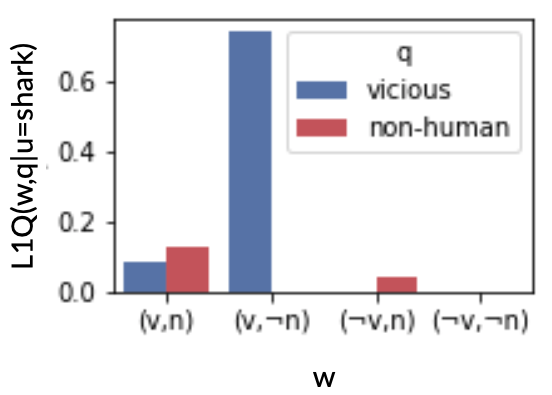
\includegraphics[width=0.5\textwidth]{images/l1posteriorquality.png}
	% \begin{subfigure}{0.5\textwidth}
	% % \centering
	% \end{subfigure}\hfill\begin{subfigure}{0.5\textwidth}
	% % \centering
	% 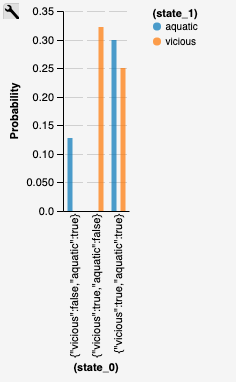
\includegraphics[width=\textwidth]{images/l1posteriorquantity.png}
	% \end{subfigure}
	\caption{Figure showing the posterior distribution of $\protect\QLONE$ on hearing \emph{shark}. $v$ and $n$ abbreviate the Boolean variables \emph{vicious} and \emph{non-human} respectively.}
	\label{fig:l1barplot}
	\end{figure}
	% change to minipage
% incorporate talk of predicates

	% but note that predicative metaphors can be treated in a similar way. 
	% We begin by describing an interpretation of $\QLONE$ where nouns and adjectives denote sets of properties, similar to the interpretation in \citep{kao}. 
		% : note that in standard compositional semantic analyses of adjectival modification, the meaning of $[a\quad n]$ is a truth-valued function on entities.
		% 	say: not as different as it seems
	% The posterior distribution of the literal listener $L_0$, which reasons about the semantics, represents the literal meaning of the AN metaphor, while $\QLONE$ has the capability of deriving a metaphorical interpretation.
		% For a given AN metaphor $[a\quad n]$, the core idea is to take $w\ in W$ to be ways that $n$ could be, and $u\in U$ to be a set of adjectives (including $a$) which could be said. Then, the posterior of $L_0$ on hearing $a$ modifying $n$ represents the literal meaning of $[a\quad n]$. The posterior of the $\QLONE$ represents the metaphorical interpretation of $[a\quad n]$.

	% In this example, $P_L$ represents the listener's prior belief about what the temper in question is like. On hearing \emph{fiery}, they update their beliefs so that the temper has all the properties denotation by the adjective. This is a literal interpretation, in that the listener now believes that the temper is both warm and intense, the two properties we take \emph{fiery} to denote for the sake of this example.
		% Note, however that the definition of $L_0$ only requires $\llbracket\cdot\rrbracket$ to be a function of type $U\to (W \to [0, 1])$, i.e. a function mapping an utterance and world to a real number $r$, with $0\leq r\leq 1$. This fact will be relevant when generalizing to a distributional semantics in section \ref{bayesdist}.
	% stuff for thesis version
	% For example, for the case of an AN metaphor like \emph{fiery temper}, states $w$ are possible ways which a temper could be. After receiving the modifier \emph{fiery}, the literal listener updates their beliefs in a way which corresponds to the meaning of \emph{fiery}.

	% In the case of metaphor, this prior will represent the listener's belief about the source of the metaphor, for example, what a temper is like
		
		% : full generality: q is an idempotent function $W\to W$


	% For instance, on hearing (\ref{met:1}), the listener can infer that Jane is hardworking, but doesn't own a gun, even though \emph{soldier} would suggest both of these attributes to a literal listener.

	% $S_1$ chooses their utterance in order to best convey which world they are in (that is, which image they have been presented with). We define $S_1$'s utility function in (\ref{utilityfunc}) and $S_1$ in (\ref{s1simplersa}):



	% \begin{exe}
	% \ex $U(u,w) = \log(L_0(w\vert u))$ \label{utilityfunc}
	% \ex $S_1(u\vert w) \propto e^{U(u,w)}$ \label{s1simplersa}
	% \end{exe}

	% $L_1$, on hearing \emph{wet}, will place more mass on \emph{fish} than \emph{shark}, which models the reasoning process described above.

			% This means that if the $L_1$ will update their prior so that the most likely world is the one corresponding to the exact height the received utterance denotes. So if the $L_1$ hears that Tarksi is 6 feet tall, they will infer that he is no more than 6 feet tall, since, if he had been, the informative $S_1$ would have said an utterance denoting a greater height. This inference corresponds to the notion of \emph{scalar implicature} - when speaking to an $L_1$ listener, it is possible to \emph{imply} that Tarski is exactly 6 feet tall by saying that he is at least 6 feet tall. Therefore the information conveyed is greater than the strict literal meaning of the utterance. 


			% For instance, suppose worlds are simply values corresponding to the height of some person, say, Alfred Tarski, and that utterances denote his height too. On hearing the utterance ``6 feet'', the literal listener will update his prior on possible worlds so that it only includes worlds in which Tarski is at least 6 feet tall.

			% The speaker, $S_1$ attempts, in turn, to produce the utterance u which maximizes a utility function U. For the simplest case of RSA, we define U as

			% % \footnote{Basic enrichments to this setup include the subtraction of a cost term from U(u$\vert$w), and a so-called ``rationality parameter'' which multiplies U(u$\vert$w).}:


			% Using the utility function in (\ref{utility}) and assuming a uniform prior on utterances, we obtain a distribution for $S_1$ proportional to the utility:
			% \begin{exe}
			% \end{exe}

			% Informally, this means that the speaker will most favor the utterance which denotes the exact height that the speaker believes Tarski to be. Any utterance denoting a lesser height will be true in our semantics and therefore will have some utility, but will be strictly less informative than saying the exact height. Importantly, utterances denoting a greater height receive no utility and are ruled out, since they would lead the $L_0$ to a world incompatible with the speaker's world. This means that it is necessary to add something to the model in order to deal with non-literal utterances (i.e. utterances which are false relative to the speaker's world).


	




	

	% \subsubsection{Interpreting $\protect\QLONE$}

	% 	this is getting so so so messy




	% \citep{kao} provides an interpretation of $\QLONE$ as follows.\footnote{The details of presentation differ somewhat from those in \cite{kao}, but is conceptually very similar.} 
	% Each $u\in U$ is a predicative metaphor composed of a subject and a predicate (\emph{Life is a journey},\emph{Time is a river}, etc).

	% We say that $\llbracket u\rrbracket(w)$ if and only if the s
	

	% In linguistic models of semantics, $\llbracket\cdot\rrbracket$ is typically a function of type $U\to (W \to \{0, 1\})$ mapping an utterance $u\in U$ to the characteristic function of the set of worlds $w\in W$ with which $u$ is compatible. 
	% RSA requires hand-constructed inputs for three aspects of the model: the semantics used in $L_0$, the set of possible utterances in $S_1$, and the set of world states in $L_0$ and $L_1$.

	% In our current example, the semantics is a mapping f the meaning of an utterance is a real number, and the possible utterances are a set of real numbers. Even here, however, it is necessary to choose some discrete set of real numbers which are valid utterances, by hand.

	% These three hand-constructed inputs are controlling factors on the scalability and domain-genericity of RSA, since each case of RSA requires the provision of all three. As we shall see, RSA with Questions under Discussion introduces a fourth such controlling factor: the need for a predetermined set of QUDs to be provided to the model.

	% The interpretation given to $\QLONE$ in \citep{kao} makes use of a very simple truth-conditional semantics

	% \footnote{The model could equally be applied to adjectival metaphors like \emph{fiery temper}, \emph{cold personality}; in this case, the analogue of the predicate is the modifying adjective}.
			
	% Each $w\in W$ is a subset of properties (for some entire set of properties $P$), representing the properties that the subject of a given metaphor has. For instance, when interpreting \emph{Time is a river}, each $w\in W$ is a possible set of the properties true of \emph{time}. For each property $p$, $q_p$ is a function which maps a set of properties $w$ to $1$ if $p\in w$, else $0$.
	% Finally, we construct a semantics $\llbracket\cdot\rrbracket$ by having each predicate denote a set of properties too, so that $\llbracket u\rrbracket(w)$ iff the denotation of the predicate is a subset of $w$.

	% the set $W_q$ of all worlds $w'$ which also contain property $p$.


	

		% a different interpretation of $\QLONE$, where $W$ is a vector space, and the semantics is not truth-conditional.


		% fiery temper



			% We suggest that the advantage that DistRSA offers over the baseline is simply the dynamics of RSA generally: the model takes into account not only the observed utterance, but possible alternatives, giving rising to an ``explaining away'' effect discussed in section (\ref{rsawithqud}). For example, the $\QLONE$ would be unlikely to infer that ``The man is a cat'' conveyed stubbornness, since ``The man is an ox.'' is an alternative which performs this task better.


	% (\cite{kao}) proposes a model of metaphors of the form ``A is a B'' in which world states are a set of Boolean properties of A. Accordingly, a listener's prior belief is their knowledge about what A is like before hearing ``B''. The model must then account for how a listener is able to hear ``A is a B'', and only update their beliefs about A with regards to certain properties of B. For instance, on hearing that the lawyer is a shark, I may conclude that the lawyer is bloodthirsty, but not that she has gray skin.  

	




	% Let us suppose that the metaphor in question is ``The lawyer is a shark.''. We first supply a prior on possible worlds (for $L_0$ and $L_1$), on QUDs for $L_1$ and on utterances for $S_1$:

	% \begin{itemize}
	% \item World Prior\footnote{The notation here of $\langle$c(lever)=True$\leftarrow\alpha$,v(icious)=True$\leftarrow\beta$,a(quatic)=True$\leftarrow\gamma\rangle$ denotes a distribution where the Boolean value for \emph{clever} is sampled a Bernoulli distribution weighted at $\alpha$ to True, and likewise, \emph{mutatis mutandis} for \emph{vicious} and \emph{aquatic}.}: 

	% \begin{itemize}

	% \item $\langle$c=True$\leftarrow$0.7,v=True$\leftarrow$0.6,a=True$\leftarrow$0.001$\rangle$
	% \end{itemize}
	% 	% \subitem $\langle$c=True,v=True,aquatic=False$\rangle$ : 0.3
	% 	% \subitem $\langle$c=True,vicious=False,aquatic=False$\rangle$ : 0.2
	% 	% \subitem $\langle$clever=False,v=True,aquatic=False$\rangle$ : 0.4
	% 	% \subitem $\langle$clever=False,vicious=False,aquatic=False$\rangle$ : 0.1
	
	% \item $Q$:
	% \begin{itemize}
	% \item \emph{clever} ($\lambda \langle x,y,z\rangle \to x$) : 1/3
	% \item \emph{vicious} ($\lambda \langle x,y,z\rangle \to y$) : 1/3
	% \item \emph{breathes-underwater} ($\lambda \langle x,y,z\rangle \to z$) : 1/3
	% % \end{itemize}
	% % \item The map from utterances to probability distributions used in the interpretation function:
	% % \begin{itemize}
	% % \item \emph{shark} : $\langle$c=True$\leftarrow$0.7,v=True$\leftarrow$0.9,a=True$\leftarrow$0.9$\rangle$
	% % \item \emph{fish} : $\langle$c=True$\leftarrow$0.5,v=True$\leftarrow$0.2,a=True$\leftarrow$0.9$\rangle$
	% \end{itemize}
	% \end{itemize}

	% We now show parts of the calculation for the $L_0$, $L_1$ and $S_1$:
	% of a particular world and QUD given that we have heard \emph{shark}. 
	% Note that we normalize at each step of the calculation ($L_0$,$S_1$,$L_1$), so that the output is a probability: 

	% Let $w_1 = \langle$ c=False,v=True,a=False $\rangle$

	% Let $w_2 = \langle$ c=True,v=False,a=False $\rangle$

	% $L_0(\emph{w_1}\vert\emph{\mathit{shark}}) = I(f,w_1)*P(f\vert \emph{\mathit{shark}})*P(w_1) = 0.143$

	% $S_1(\emph{\mathit{shark}}\vert w_1, \emph{\mathit{vicious}})$

	% $ = \frac{\sum_{w'}q(w_1)=q(w')*L_0(w'\vert \emph{\mathit{shark}})*P(u)}{\sum_u\sum_{w'}q(w_1)=q(w')*L_0(w'\vert \emph{\mathit{shark}})*P(u)}$

	% $ = 0.773 $

	% $L_1(w,\emph{\mathit{vicious}} \vert \emph{\mathit{shark}})$ 

	% $ = \frac{S_1(\emph{\mathit{shark}}\vert w_1, \emph{\mathit{vicious}}) * P(w_1) * P(\emph{\mathit{vicious}})}{\sum_{w'} S_1(\emph{\mathit{shark}}\vert w', \emph{\mathit{vicious}}) * P(w') * P(\emph{\mathit{vicious}})}$ 

	% $ = 0.094$

	% By contrast, $L_0(\emph{w_2}\vert\emph{\mathit{shark}}) = 0.016$. 

	% In other words, the model predicts, given the utterance \emph{shark}, that the lawyer is more likely vicious and not clever than the reverse. This conclusion is reached by the fact that \emph{fish} would have been a more informative utterance if w$_2$ were the speaker's world rather than w$_1$.

	% One noteworthy feature of $\QLONE$ is \emph{explaining away}. Suppose, for instance, that we add a third possible utterance to our model, \emph{fox}. Supposing that foxes are clever, the probability of the QUD being \emph{clever} when the utterance heard by the $L_1$ is \emph{shark} will decrease, in the presence of a more informative utterance for this QUD. Informally, this accords to the reasoning process: ``my interlocutor could have said \emph{fox} to express her target meaning, but she didn't, so it is less likely that she was conveying the lawyer's cleverness by saying \emph{shark}''. 

	% \subsubsection{Metaphorical modification}
	% We can also marginalize out the world variable by summing over it, to obtain a posterior on QUDs. This tells us which QUD is most likely, given that the listener heard \emph{shark}, when their prior reflected the properties of lawyers. The model correctly predicts that \emph{vicious} is the best QUD, with 0.336 of the probability mass.
	 

	% A second property of QUD RSA is that the model is asymmetric, in the sense that ``A is a B'' results in a different meaning to ``B is an A''. This is because A and B in ``A is a B'' correspond to entirely different things in the model. \emph{A} informs the listener prior, while \emph{B} is the observation on the basis of which the prior is updated to the posterior.

	% Linguistically, this asymmetry seems to be a general feature of predicative statements, and \emph{a fortiriori}, of predicative metaphors; ``The politician is a butcher.'' does not mean the same as ``The butcher is a politician.''.


	% Qualitatively, the model is able to infer QUDs for sentences like ``John is a shark.'', given a simple semantics, and sets of possible utterances and QUDs.

	% More generally, RSA models a sort of counterfactual reasoning. On hearing ``The lawyer is a shark.'', we consider what alternative utterances to \emph{shark} would have done a better job at conveying each possible world and QUD pair. 

		% explaining away: add owl: explains away clever: IMPORT EXAMPLE:
			 % As with standard RSA, distRSA exhibits an "explaining away" effect. This means that the presence of an S1 alternative can reduce probability mass for a particular QUD. More concretely, suppose we are doing L1 inference over worlds and QUDs, having heard "the man is a shark" (or rather, having started with a Gaussian prior centered at the word vector for "man", and receiving the utterance "shark"). "slippery" might be a good QUD here, in the sense that "shark" is informative about "slipperiness". However, suppose that "fish" and "snake" are both alternative utterance to "shark", in the S1. Supposing that these convey slipperiness better than "shark" does, "slippery" will be downrated as a QUD for shark. 
\section{Distributional Semantics} \label{distmods}

	From a linguistic corpus, it is possible to obtain a mapping from words to points in a high-dimensional vector space that has the property that semantic similarity of a pair of words $a$ and $b$ corresponds to a metric, such as cosine distance, between the vectors $\overrightarrow{a}$ and $\overrightarrow{b}$.

	Mappings of this sort, commonly referred to as \emph{word embeddings} or \emph{distributional models of word meaning}, can be obtained either by dimensionality reduction of a co-occurrence matrix \citep{pennington2014glove}, or by extracting the weights of a statistical model \citep{mikolov2013distributed,peters2018deep,devlin2018bert} trained on a separate task.

	In either case, word embeddings provide a way to empirically obtain fine grained connotations of lexical items \citep{mikolov2013distributed}, and have been used effectively in a number of NLP tasks \citep{dai2015semi,radford2018improving}. They have also been used to compute vectorial representations of phrases and sentences \citep{socher2013recursive, coecke2010mathematical}.
			% word embeddings appear to encode syntactic and semantic information (\citep{mikolov2013linguistic}, and as such, are useful element in many NLP tasks such as sentiment analysis \citep{socher2013recursive}.

	% (\cite{pennington2014glove}) argues that GloVe vectors exhibit a degree of linear structure, in the sense that for various quadruples of words (A,B,C,D), such that A is to B as C is to D, the corresponding pretrained vectors approximately satisfy the equation $\overrightarrow{\text{A}} - \overrightarrow{\text{B}} = \overrightarrow{\text{C}} - \overrightarrow{\text{D}}$, where $\overrightarrow{\text{A}}$ is the word vector corresponding to the word A. For instance, the nearest word vector by cosine distance to the point ($\overrightarrow{\text{king}}-\overrightarrow{\text{man}}+\overrightarrow{\text{woman}}$) in the Word2Vec embedding space is $\overrightarrow{\text{queen}}$.

		

	Metaphor is an obvious candidate for approaches that use distributional semantics: a wide variety of attempts have been made to leverage the information inherent in pre-trained word vectors for the detection, interpretation and paraphrase of metaphor (see \cite{shutova2016design} for an overview of proposed systems.).
		% TODO: needs your own citations

	Our hypothesis is that, while the information in high quality word embeddings captures important aspects of meaning, a cognitively realistic model of metaphor interpretation should also incorporate Gricean reasoning, of the sort formalized in the RSA framework. We now explain how $\QLONE$ can be combined with a distributional model of word meaning.

	% An intuition which is voiced in many of these approaches is that metaphorical predicates should agree with only certain features of the subject. For instance:
	% \begin{quote}	``Computing a meaning always involves activating context-appropriate features and inhibiting or deactivating inappropriate features.'' (\cite{kintsch})
	% \end{quote}

	% A similar point is made about adjective-noun (AN) composition by (\cite{grefenstette2013category}): 
	% \begin{quote} ``In turn, through composition with its argument, I expect the function for such an adjective to \emph{strengthen} the properties that characterise it in the representation of the object it takes as argument.''
	% \end{quote}

	% Here, Grefenstette is suggesting that an adjective A, when modifying a noun N, targets certain properties of N and not others. He exemplifies this point as follows: ``When I apply ``angry'' to ``dog'' the vector for the compound ``angry dog'' should contain some of the information found in the vector for ``dog''. But this vector should also have higher values for the basis weights of ``fighting'', ``aggressive'' and ``mean'', and correspondingly lower values for the basis weights of ``passive'', ``peaceful'', ``loves''.''

	% In the philosophical literature on metaphor, a more abstract version on this idea that only certain aspects matter is alluded to by (\cite{black}), where for a metaphor ``A is a B'', Black refers to ``A'' as the ``principal subject'' and ``B'' as the ``subsidiary subject'':
	% 		\begin{quote}
	% ``We can say that the principal subject is  ``seen through'' the metaphorical expression - or, if we prefer, that the principal subject is ``projected upon'' the field of the subsidiary subject.'' - (\cite{black})
	% \end{quote}

	% Black offers the example of the metaphorical description of a war as a game of chess, commenting that ``the chess vocabulary filters and transforms: it not only selects, it brings forward aspects of the battle that might not be seen at all through another medium''.

	% The Bayesian model of metaphor proposed by (\cite{kao}) offers a way of capturing this dynamic of caring about certain aspects of the subject and not others: in this model, a listener jointly infers a Question Under Discussion (QUD), which dictates which aspects of the modifier or predicate to care about, and a world state, based on the information about the subject. This sort of joint inference of world state and topic or QUD is absent from previous distributional approaches to metaphor.

	% Our proposal is to unite distributional semantics with Bayesian pragmatics by constructing an RSA model of metaphor which uses word vectors. In this setting, world states will become vectors in the space and QUDs will be orthogonal projections which map these vectors to vectors in subspaces of the space.

	% We now review the general RSA framework, as well as the non-literal extension to RSA (\cite{kao}) on which our model will build.
	% The work closest to this, to our knowledge, is \cite{kintsch}, which proposes a single scheme for literal and metaphorical predication.	
\section{Bayesian pragmatics with a distributional semantics} \label{bayesdist}

	The set-theoretic interpretation of $\QLONE$ takes states $w \in W$ to be sets of properties describing the source of the given metaphor, and a semantics to be a function $U\to(W\to\{0, 1\})$.
	% , projections to be surjective functions out of $W$
	% . The semantics maps utterances to functions from worlds to Boolean values, or equivalently, maps a pair $(u,w)$ to $1$ if they are compatible, and $0$ otherwise.

	We now introduce a \emph{vectorial} interpretation of $\QLONE$. Importantly, this requires no modification to equations (\ref{defl0}-\ref{defl1}). The crucial difference is that our state space $W$ is now not just a set, but a vector space determined by a word embedding $E : U\to W$, so that elements $\overrightarrow{w}\in W$ are vectors.\footnote{We note that this generalization is natural, since the set-theoretic interpretation of $\QLONE$ can be viewed as a special case of the vectorial interpretation, for a vector space over the Boolean field (rather than the real field). That is, consider an n-tuple of Booleans $w$ as a vector of $0$s and $1$s, with $P$ providing the basis of the space.} For our application of the model, we assume $U$ is a set of adjectives. 

	% given a basis set of properties $P=P_0...P_n$, a vector of $n$ 0s and 1s, with 1s corresponding to present properties and 0s corresponding to absent ones, is equivalent to a subset of $P$, i.e. the denotation of a word.} 
		

		% but we now take the denotation of a word $u$ not to be a set of properties, but rather the vector $\overrightarrow{u}$ corresponding to $u$ under a word embedding $E$.
		% As a consequence, the set of states $W$ is now infinite, consisting of all vectors in the vector space of $E$.

		% We now outline the details of the \emph{vectorial interpretation}.
	% That is, denotations of words that are sets of properties can be viewed as vectors of 0s and 1s, 
	% A projection function $q$ amounts to a linear projection in this space. 
	% in a vector space where the set of properties is a basis.
	

			% general notion of projection; idempotent function
		% but more that: given an element of W, a projection induced by that element


		% For instance, in a truth-conditional semantics, we might want to assign a truth value to \emph{John is a shark.}


		
	
				% also before: for simplicity, we assume alternative utterances with same subject
		% the set of possible utterances (\emph{The man is a shark}, \emph{})
				% the pragmatic meaning of u is a distribution over W, i.e. a distribution over points in


		% the meaning $\llbracket u\rrbracket$ of a word $w$ is a function $V\to [0,1]$





	\subsubsection{The listener's prior} 

		In the set-theoretic interpretation of $L_1^Q$, with finite $W$, a discrete prior $P_L$ over $W$ sufficed. In the present case, where $W$ is necessarily infinite (ranging over all real-valued vectors), we use a multivariate spherical Gaussian distribution, which can be parametrized by a vector $\overrightarrow{\mu}$ for the mean and a single scalar $\sigma$ (the value of every diagonal entry of the covariance matrix). We define the prior over projections $P_{L_Q}$ to be uniform.

		\begin{exe}
		\ex $P_L(w) = P_{\mathcal{N}}(w\vert\mu=E(\textrm{\emph{target}}),\sigma=\sigma_1)$ \label{vect:prior}
		% \overrightarrow{\mathit{source}}
		\end{exe}

		We can view $P_L$ as representing uncertainty over the position of the entity or concept that the target noun (e.g. \emph{man} in ``The man is a shark'') represents.
		% \footnote{Note that this prior does not represent lexical uncertainty over the meaning of the subject word, but rather uncertainty over what the entity or concept that the subject denotes is like.} 
		The goal of the speaker is to convey a position in the space 
		% (which they think represents the nature of the source noun's denotation) 
		to the listener, and the goal of the listener is to infer what this position is. In this sense, a spatial reference game is being played  \citep{golland2010game}, in an abstract word embedding space.\footnote{Our vectorial semantics bears comparison to the \emph{conceptual space} semantics of \citet{gardenfors2004conceptual}, as well as the proposal for metaphor comprehension offered by \citep{kintsch2000metaphor}.}

				% are near $\llbracket\mathit{time}\rrbracket$
		
		


		The multidimensional Gaussian distribution weights most heavily those points nearest to its mean. By setting the mean of the prior as $E$(\emph{target}), we encode the listener's assumption that the meaning the speaker wishes to communicate is in the neighborhood of the source noun. $\sigma_1$ is a hyperparameter of the model.

			% , e.g. $\overrightarrow{\text{temper}}$ for the metaphor \emph{fiery temper}. The points in the distribution represent meanings of \emph{temper} that might not be encoded in its vector. For instance, some points in the distribution might be closer to $\overrightarrow{\text{intense}}$ or $\overrightarrow{\text{unstable}}$. 

		 % of the metaphor, we represent the listener's prior uncertainty over what the subject is like, or equivalently, what point in the space the subject occupies.
			
			% On hearing 

			% Updating one's prior on what time is like, namely the Gaussian centered on $\overrightarrow{\text{time}}$ so that these points have more weight, represents in this model an update regarding one's knowledge about time.

	\subsubsection{The semantics}


			% This is unsurprisingly, given that the relational interpretation of $\QLONE$ amounts to the vectorial interpretation, but for a vector space  over the Boolean field, rather than the real field.

		A word embedding space has no explicit representation of truth. That is to say, while we can compare the similarity of a noun and an adjective according to a variety of metrics, we do not have a means of categorically determining the compatibility of that adjective and noun.

		As far as our model is concerned, this is not a problem since the definition of $L_0$ in (\ref{defl0}) requires only that the semantics $\llbracket \cdot \rrbracket$ be a function $U\to (W\to \mathbb{R})$. We can define such a function as follows, with $\sigma_2$ as a hyperparameter:
		\vspace{-1.5em}
		\begin{exe}
		\ex $\llbracket u\rrbracket(w) = P_{\mathcal{N}}(w\vert\mu=E(\textrm{\emph{source}}),\sigma=\sigma_2)$ \label{vect:sem}
		% \overrightarrow{\mathit{predicate_u}}
		\end{exe}

		% However, despite the ``softness'' of a distributional meaning, will find that it is possible to use it to obtain a semantics capable of underlying $\QLONE$, 

		% since the $L_0$ requires only that the semantics be real-valued.



		The result of this definition is that the value of $\llbracket u\rrbracket(w)$ is a real number which decreases with the Euclidean distance between $u$ and $w$. 
		The advantage of defining a semantics in this way is that both the prior of $L_0$, shown in (\ref{vect:prior}) and the likelihood, namely the semantics shown in (\ref{vect:sem}), have the form of Gaussian distributions, which allows for a closed form solution of $L_0$. 
		% As with the definition of the prior in (\ref{vect:prior}), the semantics introduces a hyperparameter, namely $\sigma_2$.

	\subsubsection{Projections} 

		\begin{figure}
		\centering
			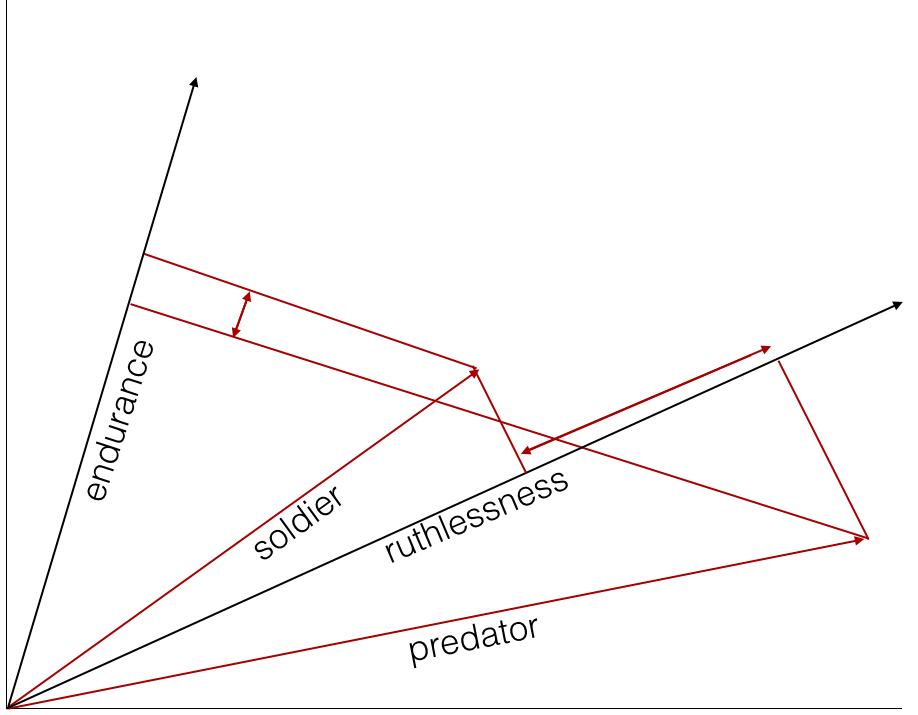
\includegraphics[height=5.5cm]{images/diagram2.png}
			\caption{In this hand-constructed 2D example, vectors for $\protect\overrightarrow{soldier}$ and $\protect\overrightarrow{predator}$ are mapped onto subspaces given by $\protect\overrightarrow{endurance}$ and $\protect\overrightarrow{ruthlessness}$.}
			% In this 2D example, the vectors for \emph{endurance} and \emph{ruthlessness} each parametrize a projection mapping all the points in the space (such as \emph{Jane} and \emph{John}) to new points. These new points can be thought of as the positions of \emph{John}, \emph{Jane} and so on in a new space which cares only about the position of the points with respect to $\protect\overrightarrow{endurance}$ or $\protect\overrightarrow{ruthlessness}$.
			\label{fig:1}
		\end{figure}
		% Since, in a distributional setting, the axes of a world state vector do not neatly correspond to its attributes\footnote{If our space was formed by a basis of co-occurrence vectors, each word would be a dimension, but this is not the case in typical word embedding spaces, the dimensions of which are much fewer than the size of the vocabulary.}, our distributional  cannot simply be a projection along an axis. 

		Finally, we need to supply an notion of a projection function $q$ that is defined on our vector space, and to specify a set $Q$ of such projections. 
		For this, we use linear projections\footnote{To see why this is the natural analogue of the projection functions used in the set-theoretic interpretation of $\QLONE$, note that when viewed as vectors in a vector space over the Boolean field, projection functions are precisely linear projections. Alternatively, note that in either case, projections $q$ are idempotent maps $(W\to W)$.} along a vector (or hyperplane) $\overrightarrow{v}$ 
		% This is a linear transformation from $W$ to the subspace given by $\overrightarrow{v}$, 
		capturing the degree to which each $\overrightarrow{w}$ extends along $\overrightarrow{v}$, ignoring orthogonal dimensions. Geometrically, it can be thought of as dropping a line from an input vector $\overrightarrow{w}$ at a right angle onto $\overrightarrow{u}$, as depicted in figure \ref{fig:1}.

			% Alternatively, note that 
				% Put another way, the definition of a projection on an object $X$ as an idempotent morphism $X\to X$, generalizes both cases. 
				% ok yes this is deeply unnecessary


				% World states and word denotations in  RSA, as described in (\cite{kao}), can already be understood as vectors over the set of two elements, \{0,1\}, or equivalently as relations between the subject and predicate. (For instance, suppose the meaning of \emph{shark} is $<$vicious=True,aquatic=False$>$. This can be rewritten as the vector $<$1,0$>$.) The intuition behind our model is to generalize QUD RSA to a vector space over the reals.
		% As in the set-theoretic interpretation, w
		In practice, we restrict ourselves to projections along a vector, rather than a larger subspace. 
		% However, we no longer have an obvious set of projections $Q$, corresponding to an explicit set of properties $P$. This is because the basis vectors of a word embedding space such as GloVe or Word2Vec do not correspond to easily interpretable attributes of the words in the space.
		To obtain a set $Q$ of projections, we first note that since the denotations of words are vectors in $W$, any word parametrizes a linear projection $q$. For instance, we can think of the word \emph{vicious} as parameterizing a \emph{viciousness} projection, which measures how far the denotations of all other points in the space fall along $\overrightarrow{\mathit{vicious}}$. 
		We choose $Q$ as a set of gradable adjectives, so that the projection of a noun $n$ onto $\overrightarrow{v}$ amounts to asking: to what extent is $n$ $v$? 


					% For this reason, the natural implementation of a QUD in a vector space is as an orthogonal projection, parametrized by some hyperplane, which maps from the full space to a lower dimensional subspace. The simplest case is of a 1 dimensional projection, a line: here, every point in the original space is dropped in a perpendicular fashion onto the line. In the more general multidimensional case, given a hyperplane in our space we can obtain a function mapping points in the space to new positions, derived by dropping them perpendicularly onto the hyperplane. This projection is a linear transform to a subspace of the original vector space, pictured below in two dimension, for two word vectors, and two potential projection vectors (which here also correspond to words):

		% What set of linear projections $Q$ should we choose? In the set-theoretic interpretation, $Q$ was simply the set of all one-dimensional projections, or equivalently, projections onto each of the natural basis vectors. In the word embedding case, however, the basis vectors of a word embedding $E$ have no simple interpretation as properties.


		% As such, we can specify $Q$ as a set of words. In general, 
		% We discuss the exact choice of $Q$ in section \ref{exp}.


		% The assumption that appropriate projections exist is based on the much observed linear substructure of word embeddings, which amounts to the claim that word vectors can be roughly decomposed as a sum of a set of other word vectors. 
		% While this linearity is very noisy, we find that it suffices for our purposes

		% In non-distributional RSA, the $L_0$ prior on worlds is a uniform distribution over the finite set of possible worlds. For DistRSA, we have an infinite set of possible worlds, corresponding to the points in the word embedding space. Since we want to use to information encoded in the subject of a metaphor (e.g. ``The lawyer'' in ``The lawyer is a shark.''), we do not want a uniform distribution over these points.

		% Thus, for a metaphor, such as ``Time is a river.'', we define the listener's prior as a multidimensional Gaussian distribution centered around the word vector for \emph{time}. The choice of a Gaussian is made for two reasons: firstly, they are well-behaved mathematically, and allow us to calculate the $L_0$ distribution analytically, which is necessary for our computational model. Secondly, as discussed in section (\ref{distmods}), the GloVe word encodes semantic similarity roughly as cosine distance in the embedding space. 

		
			

		


		% Transferring RSA, specifically QUD RSA, to a distributional semantics requires the provision of analogues for the key elements of the QUD RSA model, namely:

		% 	\begin{itemize}
		% 	\item Word Denotation
		% 	\item World State
		% 	\item QUD
		% 	\end{itemize}

			% In each case, there is a natural way to enrich QUD RSA into a distribution setting. Word denotation, as we would expect, is given by the word vector corresponding to the word in question, as supplied by a pre-trained word embedding. We use the 50 dimensional version of GloVe\footnote{In general, we are agnostic as to the appropriate choice of word embedding space.}. The meaning of a word, in this paradigm, is a point in this 50 dimensional space.

			% We treat the world state as a point in this space too. Note that in both distributional and non-distributional QUD RSA, the world state and the word denotation are of the same type as each other.

		

		% The final ingredient necessary to adapt QUD RSA to a distributional setting is the notion of QUD. Recall that the QUD in the non-distribution model maps from worlds to sets of worlds which agree on a particular part of the world state. 




		% Again, it is worth noting the similarly of the simple and distributional notions of QUD. In both cases, the QUD discards information, via a many-to-one mapping from worlds to sets of worlds\footnote{This is true in the distributional case because the projection  maps more than one point to a single point. Thus, we can recast the projection as a function P from a point v to the inverse image of P(v).}.

		% \begin{figure}[htbp]
		% \hspace*{-2.5cm}                                                           
		   
		%   \caption{Projection}
		%   \label{fig:proj}
		% \end{figure}



		


		% \subsubsection{The Bayesian agents in a distributional setting} 
		% say something about the agents
		% 		Interpretation of an utterance still amounts to the updating of a prior to a posterior distribution
		% 		Intuitively, this corresponds to moving prior towards vec(utterance)
		% 	% We can think of 
		% 	s1 as informative along dimension
		% 	l1 as before
		% 		Another way of thinking of DistRSA is as a spatial reference game (e.g. \cite{golland2010game}), played in a word vector space. In this setting, the $S_1$ has knowledge of what lawyers (or a particular lawyer) is like, represented by a position of the lawyer in the vector space. They also have a QUD that they care about. They choose the noun which best conveys the known position of \emph{lawyer} with respect to the QUD in question.


				% we condition on the likelihood of the $S_1$ world state being drawn from the $L_0$ posterior after having heard any given possible utterance.
\section{Inference} \label{technicaloverview}


	% Calculating the posterior of $\QLONE$ given an utterance $u$ is far more difficult in the vectorial interpretation than the set-theoretic one. 
	Because $P_L(w)$ is a continuous distribution in the vectorial interpretation of $\QLONE$, inference by enumeration is no longer possible, and either analytic or approximate methods are required. We employ a mix of the two; the $L_0$ and $S_1$ posteriors can be calculated analytically, while $\QLONE$ requires us to develop an approximate inference algorithm.\footnote{Inference for all our models is implemented in Tensorflow, and will be made publicly available.} We describe this algorithm in parts, working up from the $L_0$.

	\begin{figure}[htbp]
	\centering
	% \hspace*{-2.5cm}                                                           
	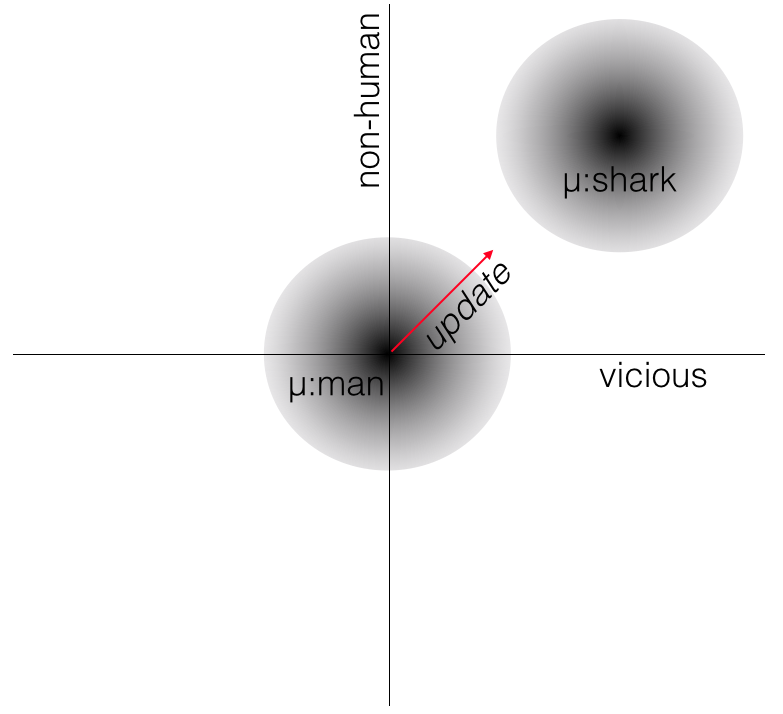
\includegraphics[height=6.5cm]{images/diagram1.png}
	   
	  \caption{2D depiction of vectorial $L\protect_0$, for $\protect\overrightarrow{man}$ = (0,0) and $\protect\overrightarrow{shark}$ = (1,1).}
	  \label{fig:2d}
	\end{figure}
	% While the general format of our model is analogous to previous models in the RSA paradigm, the vectorial setting produces a number of challenges which require novel solutions.

	% Moreover, previous implementations of RSA have employed prior distributions for both the speaker and listener with finite support. As a result, it is possible in standard RSA to perform exact inference for the $L_0$, $S_1$ and $L_1$. By contrast, our prior is a Gaussian and as such cannot be computed via exact inference, due to the need to calculate a normalizing term which sums (or rather integrates) over an infinite set. 
	% Furthermore, nesting causes approximate inference in the form of Markov Chain Monte Carlo to be unstable (see \cite{rainforth2016pitfalls}).
	% We therefore compute the $L_0$ and $S_1$ posteriors analytically, and use perform appromixate inference only at the $L_1$ level. We now describe how each of $L_0$, $S_1$ and $L_1$ is computed.
\subsubsection{L\textsubscript{0} Inference}


	Intuitively, the vectorial interpretation of $L_0$ amounts to the process shown in figure \ref{fig:2d}, where a ball, corresponding to the prior, is moved in the direction of the point corresponding to the received utterance. To calculate $L_0$ analytically, we make use of Gaussian conjugacy. When the prior $P_L$ is defined as in Equation \ref{vect:prior}, and the semantic interpretation is defined as in Equation \ref{vect:sem}, then conjugacy implies that the listener posterior is given by:

	 \begin{exe}
	\ex $L_0(w|u) = P_{\mathcal{N}}(w\vert\mu=\frac{\sigma_1^2 \sigma_2^2}{\sigma_1^2+\sigma_2^2}\cdot(\frac{{\textrm{\emph{E(target)}}}}{\sigma_1^2}+\frac{{\textrm{\emph{E(source)}}}}{\sigma_2^2}), \sigma=\frac{\sigma_1^2 \sigma_2^2}{\sigma_1^2+\sigma_2^2})$  \label{eq:L0-inference}
	 \end{exe}





	% This is the property that a distribution of the form $P_{\mathcal{N}}(w\vert\mu=subject,\sigma=\sigma_1)P_{\mathcal{N}}(w\vert\mu=u,\sigma=\sigma_2)$



	% Recall that $L_0$ is defined as follows, where \emph{subject} is the word being predicated (e.g. ``lawyer'' in ``The lawyer is a shark''):



	% \begin{exe}

	% \ex $L_0(w\vert u) \propto P_{\mathcal{N}}(w\vert\mu=subject,\sigma=\sigma_1)P_{\mathcal{N}}(w\vert\mu=u,\sigma=\sigma_2)$ \label{term}

	% e^f$ * e$^\mu$ \label{term}

	% \end{exe}

	% The left hand term represents the prior on the world state, and the right hand term represents the observation. By the self conjugacy of Gaussians, (\ref{term}) can be reduced analytically to a single Gaussian.

	% 	 citation?
\subsubsection{S\textsubscript{1} Inference}
		The speaker is defined by Equation \ref{defs0}, which in the continuous case can be rewritten as:
		\begin{exe}
		\ex $S_1(u\vert w,q) \propto \int_{w'} \delta_{q(w)=q(w')} \cdot L_0(w'\vert u)$
		\end{exe}
		This integral is computing the marginal probability of $w_q$, the projection of world $w$ onto QUD vector $q$. From Equation \ref{eq:L0-inference}, $L_0(\cdot \vert u)$ is a normally distributed random variable, and therefore projection of this random variable onto a linear subspace is also normally distributed, providing a closed-form solution to $S_1$.

		% We refer to the hyperplane which parametrizes the QUD projection as $\overrightarrow{\text{q}}$, and abuse notation by having q(v) denote the vector resulting from a projection of v along q. Note that q(v) could either be represented in the dimensionality of the original space or the projection subspace. We will assume the former, so that if v $\in$ {\rm I\!R}$^n$, q(v) $\in$ {\rm I\!R}$^n$. Then our $S_1$ is almost identical to the plain QUD RSA model:



		% \begin{exe}

		% \ex U(u,w,q) = $\log(\int_{w'} \delta_{q(w)=q(w')} * L_0(w'\vert u))$

		% \ex S$_1(u\vert w,q) \propto e^{U(u,w,q)}$

		% \end{exe}
\subsubsection{L\textsubscript{1} Inference}





	\begin{figure}

	\centering

	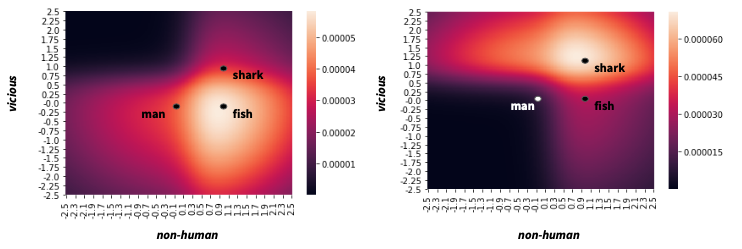
\includegraphics[width=\textwidth]{images/bothheatmaps.png}

	% \begin{subfigure}{0.5\textwidth}

	% \centering

	% 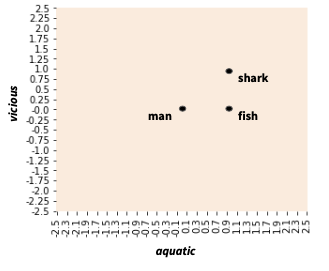
\includegraphics[width=0.85\textwidth]{images/denotations.png}

	% \end{subfigure}\hfill\begin{subfigure}{0.5\textwidth}

	% \centering

	% 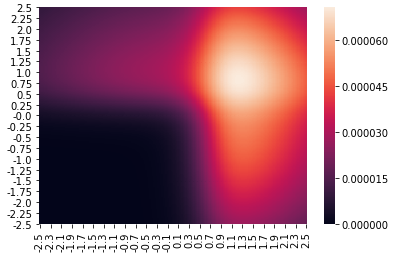
\includegraphics[width=\textwidth]{images/discretel1heatmap.png}

	% \end{subfigure}

	\caption{Heatmaps visualizing the inferred $\protect\QLONE$ marginal posterior over worlds given \emph{fish} (left) and \emph{shark} (right), with $U = \{$\emph{man}, \emph{shark}, \emph{fish}$\}$, hand-chosen denotations overlaid, and $\protect\sigma\protect_1=5.0, \protect\sigma\protect_2=0.5$.}

	% Comparison between the $\protect\QLONE$ posterior under our inference algorithm (left) and under the true posterior (right), which is calculable in this two dimensional case (up to discretization of the space).

	\label{l1heatmaps}

	\end{figure}



	% \begin{figure}

	% \centering

	% \begin{subfigure}{0.5\textwidth}

	% % \centering

	% 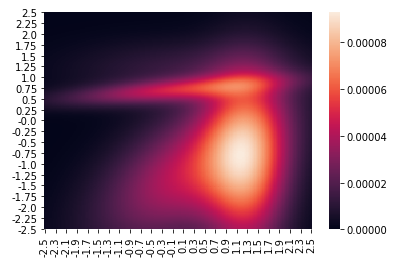
\includegraphics[width=\textwidth]{images/coolmixturel1heatmap.png}

	% \end{subfigure}\hfill\begin{subfigure}{0.5\textwidth}

	% % \centering

	% 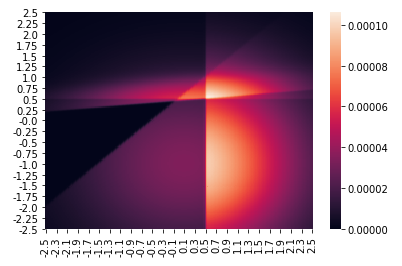
\includegraphics[width=\textwidth]{images/cooldiscretel1heatmap.png}

	% \end{subfigure}

	% \caption{ Comparison between the $\protect\QLONE$ posterior under our inference algorithm (left) and under the true posterior (right), which is calculable in this two dimensional case (up to discretization of the space).}

	% \label{l1heatmaps}

	% \end{figure}



	% caption: 

	% 	heatmaps showing...

	% 	an example of the difference between the $\protect\QLONE$ posterior under our inference algorithm and under the true posterior, in a two dimensional case where a (discretized) exact posterior can be computed exactly.

	% 	this compares our inference algorithm (left) to an exact (discretized) inference in a tractable 2 dimensional case, for the metaphor: BLAH 

	% 	with the following hand-specified word embeddings.





	% caption:

	% 	heatmaps showing the l1 inference. 

	% 		scalar implicature means that...

	% We devise the following approximate inference algorithm.



	The $L_1$ posterior is a joint distribution over one continuous and one discrete random variable. 
	% Unlike $L_0$, we are unable to use conjugacy to compute it analytically.
	Because of the linear structure of the problem, we are able to devise a near-exact inference algorithm for the marginal distribution over QUDs in $Q$, derived as follows:



	%\footnote{We verify the correctness of this algorithm in the 2 dimensional case by comparison to the exact posterior, which is calculable (up to discretization of the prior) in 2 dimensions.}



		% Moreover, we find that Mean Field Variational Inference  CITATION is not well suited

		% 	since the posterior is non-Gaussian (see figure \ref{l1heatmaps}).



	% \begin{align}

	% L_1(w,q | u) &= \frac{P(w)P(q)S_1(u|w,q)}{\sum_{q'} \int_{w'} P(w')P(q')S_1(u|w',q')} \\

	% &= \frac{P(w)P(q)S_1(u|w,q)}{K} 

	% \end{align}









	% To compute the marginal distribution over QUDs:



	 \begin{align}
	 \begin{split}
	&L_1(q | u) = \int_{\mathbb{R}^n}L_1(w,q | u) dw
	= \frac{1}{K}P_{L_Q}(q) \int_{\mathbb{R}^n}P_L(w)S_1(u|w,q) dw \\
	&= \frac{1}{K}P_{L_Q}(q) \int_{\mathbb{R}^n}P_L(w_q, w^\bot)S_1(u|w_q,q) dw
	= \frac{1}{K}P_{L_Q}(q) \int_{\mathbb{R}^n}P_L(w_q) P_L(w^\bot)S_1(u|w_q,q) dw \\
	&= \frac{1}{K}P_{L_Q}(q) \int_{Q^\bot}P_L(w^\bot) dw^\bot \int_{Q}P_L(w_q) S_1(u|w_q,q) dw_q \\
	&= \frac{1}{K}P_{L_Q}(q)  \int_{Q}P_L(w_q) S_1(u|w_q,q) dw_q\nonumber
	\end{split}
	 \end{align}
	



	Here $K$ is a normalizing constant, $w, q\in \mathbb{R}^n$, and $w_q$ is the projection of $w$ onto the vector $q$. $Q$ is the subspace of $\mathbb{R}^n$ spanned by the vector $q$, and $Q^\bot$ is the orthogonal complement of $Q$. 
	The vector $w^\bot$ is the projection of vector $w$ onto the subspace $Q^\bot$. The final equation is a one-dimensional integral, and can be computed using a discrete approximation.\footnote{We use a Gaussian approximation, which easily generalizes to the setting of multi-dimensional QUDs.} The constant $K$ can be found from the constraint $\sum_q L_1(q|u) = 1$. 

	Figure \ref{l1heatmaps} provides a visualization of the $\QLONE$ posterior in a simple 2D case corresponding to the example used for the set-theoretic example in figure \ref{fig:l1barplot}.


		% To compute the joint posterior over $W$ and $Q$, we first compute the conditional posterior $P(w|q,u)$ for each $q\in Q$, and then determine the marginal posterior on $Q$, $P(Q)$  HOW THO? 

		

		% fixing a particular projection $q$, we can compute the conditional probability of $w$ 
			% for an orthonomal basis of $W$ including $q$, the mean and variance of this posterior is the same as the prior in every dimension except $q$. 
			% 	In the single dimension of interest, we approximate the conditional posterior by performing gradient descent to find the mean of the posterior, and discretizing the now one-dimensional prior. 





	% $L_1$ is defined as follows, where P$_{QUD}$ represents the prior on QUDs. As discussed below, we can either have this be a continuous distribution over hyperplanes corresponding to projection functions, or a discrete distribution of hyperplanes corresponding to a set of n-tuples of words. In either case, we assume it is a uniform distribution:
	% \begin{exe}
	% \ex $L_1(w,q\vert u) \propto S_1(u\vert w,q) P_{\mathcal{N}}(w\vert\mu=subject,\sigma=\sigma_1)*P_{QUD}(q)$
	% \end{exe}
	% While we were able to use analytic methods to derive the $L_0$ and $S_1$ posteriors, we cannot do so for the $L_1$. Instead, we must use an approximate inference method. We try two different inference algorithms, Hamiltonian Monte Carlo (\cite{neal2011mcmc}), a brand of Markov Chain Monte Carlo inference algorithm which makes use of gradient information to move from one sample to the next, and Variational Mean Field inference (see \cite{blei2017variational}), an optimization based inference algorithm. In our first experiment we use the former, while we make use of the latter in our second, on account of its speed.

	% Variational Inference (VI) greatly increases efficiency over other inference methods, at the cost of requiring gradients for the $S_1$ and the functions the $S_1$ calls. Fortunately, it is possible for us to calculate these gradients, using automatic differentiation.

	% $L_1$ performs joint inference over QUDs and worlds. While the nature of the prior over worlds has already been discussed, two variants of $L_1$ are possible, as regards to prior on QUDs. The first is to have a categorical distribution over a set of projection hyperplanes (QUDs), for example those corresponding to n-tuples of words, according to the pretrained embedding. The output of our inference then gives us a categorical distribution over QUDs, corresponding to words (as well as a continuous distribution over worlds). 

	% The second variant is to have the QUD be a continuous variable. As a result of the way the projection is defined, only the angle and not the magnitude of the projection hyperplane matters. As such, we can have a uniform prior over unit hyperplanes. We will refer to these as two models as the Categorical and Non-Categorical $L_1$, respectively.

	% The advantage of the Categorical $L_1$ is that we can choose a particular set of QUDs, for instance, the vectors corresponding to a given set of words, and weight this prior according to the frequency of these words. This allows us to supply our model with a set of possible QUDs, and have it return a categorical distribution over them, as the $L_1$ QUD posterior.

	% The Non-Categorical model, on the other hand, has the contrasting benefit that no set of possible QUDs need be provided to the model. Furthermore, the use of Hamiltonian dynamics for performing the joint inference results in much faster performance. However, the Non-Categorical model yields significantly less stable results, and as such, we use only the Categorical model in our experimentation.
% \vspace{2em}
\subsection{Interpreting results from $\protect\QLONE$}

	We now have an algorithm for approximating the posterior distribution of $\QLONE$ after hearing a metaphor $u$. We convert this into an interpretable prediction by selecting the adjectives $q\in Q$ which have high probability under the marginal posterior distribution over $Q$ as interpretations of the metaphor.
	 % $u$ that the model considers likely. 

	% This completes the specification of the vectorial interpretation of $\QLONE$. In this setting, $\QLONE$ receives an utterance $u$ (e.g. \emph{Time is a river.}) and returns a joint distribution, assigning a probability to each pair $(q,w)\in QxW$. 


	% For example, on the metaphor, (subject=\emph{man}, predicate=\emph{shark}), the 
	% 	blah with most mass
		% TODO example

	% Qualitatively, these results are promising: for the most part, the projections identified seem appropriate. Note that the projection should not be taken as a paraphrase of the metaphorically used noun. For instance, \emph{tame} is a suitable projection for ``The man is a lion.'', because tameness is a topic that the use of the metaphor resolves, even though lions are the opposite of tame. 
\section{Experimental Evaluation} \label{exp}

	In order to test our model on human judgments, we design an experiment which compares the $\QLONE$ interpretations of metaphors to a baseline model which uses word embeddings but no pragmatic reasoning.


	\subsubsection{Experimental Design}

		\begin{figure}
		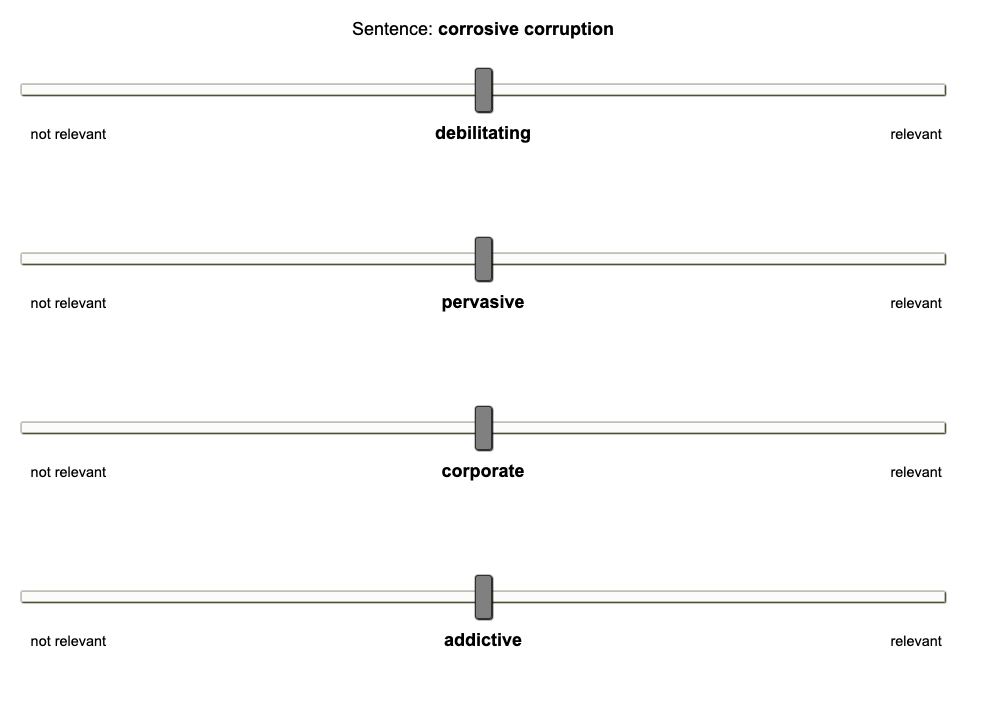
\includegraphics[height=8.5cm]{images/slide.png}
		\caption{An item in the experiment. Item order, and in-item order of the 4 adjectives from $\protect\QLONE$ and baseline models is randomized.}
		\label{fig:slide}
		\end{figure}

		\begin{figure}
		\begin{subfigure}{0.3\textwidth}
			\begin{center}

			\setlength\extrarowheight{-10pt}
			\renewcommand{\arraystretch}{0.1}
			\begin{tabular}{ c | c | c  }
			 \tiny $\protect\QLONE$ adjectives & \tiny BASELINE adjectives & \tiny metaphor \\ 
			\hline
			 % cell4 & cell5 & cell6 \\ 
			 % $\protect\QLONE$ adjectives & BASELINE adjectives & metaphor \\
			\tiny undistorted, faceless & \tiny wolfish, pitiless & \tiny cut-throat competition\\
			\tiny euphoric, giddy & \tiny despondent, chagrined & \tiny deflated emotions\\
			\tiny greater, moral & \tiny alarming, impoverished & \tiny deeper poverty\\
			\tiny traditional, fresh & \tiny homemade, organizational & \tiny corporate pie\\
			\tiny imminent, speculative & \tiny recessionary, substantial & \tiny economic meltdown\\
			\tiny evil, suicidal & \tiny angry, nasty & \tiny blind hate\\
			\tiny stellar, untold & \tiny humiliating, regional & \tiny economic heap\\
			\tiny unbearable, mental & \tiny afflicted, worse & \tiny debilitating poverty\\
			\tiny bipartisan, anti & \tiny political, affordable & \tiny economic prescription\\
			\tiny quiet, idyllic & \tiny important, everlasting & \tiny deserted friendship\\
			\tiny beautiful, particular & \tiny fearful, sincere & \tiny blue feelings\\
			\tiny unproductive, crummy & \tiny ungodly, undoable & \tiny backbreaking rent\\
			\tiny dangerous, possible & \tiny alleged, guilty & \tiny criminal path\\
			\tiny cynical, vulgar & \tiny lustful, insatiable & \tiny dirty desires\\
			\tiny difficult, obvious & \tiny preliminary, analytical & \tiny deep analysis\\
			\tiny easy, traditional & \tiny possible, social & \tiny economic pie\\
			\tiny successive, miserable & \tiny fiscal, brutal & \tiny crushing unemployment\\
			\tiny wrong, new & \tiny warmer, appropriate & \tiny cold justice\\
			\tiny refreshing, copious & \tiny unopened, divine & \tiny bottled passion\\
			\tiny awash, treacherous & \tiny undulating, unprecedented & \tiny crisscrossed chaos\\
			\tiny jubilant, galvanized & \tiny buoyant, wobbly & \tiny deflated pride\\
			\tiny desirable, modest & \tiny residential, fragile & \tiny durable middle-class\\
			\tiny amusing, cynical & \tiny nasty, afraid & \tiny biting look\\
			\tiny recent, likely & \tiny slight, annual & \tiny economic rise\\
			\tiny enduring, rich & \tiny afflicted, global & \tiny deep poverty\\
			\tiny gifted, renowned & \tiny illiterate, national & \tiny blind elite\\
			\tiny federal, necessary & \tiny southern, aggressive & \tiny economic force\\
			\tiny cyclical, breakneck & \tiny zippy, sluggish & \tiny economic laggard\\
			\tiny immense, intellectual & \tiny overall, analogous & \tiny economic sphere\\
			\tiny precarious, creaking & \tiny adequate, prolonged & \tiny collapsing health\\
			\tiny stale, unrealistic & \tiny wobbly, metaphorical & \tiny deflated meaning\\
			\tiny optimal, budgetary & \tiny potential, adequate & \tiny balanced growth\\
			\tiny entrepreneurial, greater & \tiny agile, possible & \tiny economic mobility\\
			\tiny wicked, dishonest & \tiny virtuous, righteous & \tiny dirty deeds\\
			\tiny cultural, genuine & \tiny astonishing, parliamentary & \tiny democratic vitality\\
			\tiny rewarding, excess & \tiny dry, lavish & \tiny draining expense\\
			\tiny vibrant, medieval & \tiny worse, grotesque & \tiny economic tapestry\\
			\tiny relentless, debilitating & \tiny battered, periodic & \tiny crushing cycle\\
			\tiny conquering, immense & \tiny embarrassing, overwhelming & \tiny crushing difficulty\\
			\tiny academic, practical & \tiny advanced, recent & \tiny economic medicine\\
			\tiny pessimistic, bleak & \tiny worried, serious & \tiny clouded future\\
			\tiny ambitious, vibrant & \tiny strategic, postwar & \tiny economic revitalization\\
			\tiny accidental, divergent & \tiny unspoken, intolerable & \tiny colliding contradiction\\
			\tiny appalling, wretched & \tiny alarming, inhuman & \tiny dehumanizing poverty\\
			\tiny overblown, depressing & \tiny bizarre, depressed & \tiny deflated joke\\
			\tiny alone, unclear & \tiny male, additional & \tiny dead money\\
			\tiny enduring, evident & \tiny homogeneous, big & \tiny deep inequality\\
			\tiny supreme, founding & \tiny constitutional, socialist & \tiny dissolved time\\
			\tiny longstanding, unshakeable & \tiny baneful, underlying & \tiny deep-rooted belief\\
			\tiny ambitious, innovative & \tiny outspoken, risky & \tiny aggressive program\\
			\tiny unchecked, continual & \tiny phenomenal, zippy & \tiny breakneck expansion\\
			\tiny rampant, worsening & \tiny acute, fatal & \tiny chronic poverty\\
			\tiny immediate, immense & \tiny atomic, illegal & \tiny economic destruction\\
			\tiny unable, wrong & \tiny heavy, anxious & \tiny broken hope\\
			\tiny internal, sustained & \tiny neurological, apparent & \tiny economic muscle\\
			\tiny inherent, legitimate & \tiny ancient, glaring & \tiny cultural impediment\\
			\tiny ideological, fiscal & \tiny philosophical, administrative & \tiny academic gap\\
			\tiny good, higher & \tiny poor, efficient & \tiny durable class\\
			\tiny worsening, prevalent & \tiny adverse, global & \tiny acute poverty\\
			\tiny successive, heartbreaking & \tiny aggravated, gigantic & \tiny crushing neglect\\
			\tiny unrelenting, magnificent & \tiny windy, torrid & \tiny blazing desolation\\
			\tiny moral, secular & \tiny parliamentary, flexible & \tiny civic fabric\\
			\tiny interactive, competitive & \tiny nonlinear, real & \tiny dynamic company\\
			\tiny principled, definite & \tiny lasting, flexible & \tiny clear-cut solution\\
			\tiny subsidized, costly & \tiny senior, insolvent & \tiny burdened service\\
			\tiny unsustainable, voluminous & \tiny macroeconomic, insufficient & \tiny ballooning expenditure\\
			\tiny lonely, idyllic & \tiny monogamous, featureless & \tiny deserted relationships\\
			\tiny disoriented, contorted & \tiny unexplored, undulating & \tiny choked gullies\\
			\tiny conquering, heartbreaking & \tiny appalling, gigantic & \tiny crushing misery\\
			\tiny dramatic, depressing & \tiny recent, greater & \tiny economic slide\\
			\tiny quiet, nondescript & \tiny forlorn, patterned & \tiny blue obscurity\\
			\tiny foreseeable, pessimistic & \tiny windless, worrisome & \tiny cloudy prospect\\
			\tiny pervasive, debilitating & \tiny addictive, corporate & \tiny corrosive corruption\\
			\tiny widespread, alarming & \tiny abject, escalating & \tiny acute ignorance\\
			\tiny flamboyant, humorous & \tiny multicolored, garish & \tiny colorful personality\\
			\tiny certain, other & \tiny painful, huge & \tiny deep rank\\
			\tiny minor, whole & \tiny good, numerous & \tiny broken melody\\
			\tiny optimistic, generous & \tiny national, ambitious & \tiny compassionate budget\\
			\tiny provocative, unflattering & \tiny memorable, charming & \tiny colorful remark\\
			\tiny feudal, authoritarian & \tiny great, aristocratic & \tiny backward tradition\\
			\tiny civil, disastrous & \tiny sluggish, allied & \tiny economic battle\\
			\tiny consequent, structural & \tiny apparent, freshwater & \tiny ecological collapse\\
			\tiny terrible, oppressive & \tiny absolute, innate & \tiny crushing ignorance\\
			\tiny potential, tremendous & \tiny ready, mild & \tiny big weakness\\
			\tiny unbearable, nagging & \tiny escalating, playful & \tiny crippling awkwardness\\
			\tiny impoverished, prone & \tiny parallel, important & \tiny backward area\\
			\tiny scientific, theoretical & \tiny potential, advanced & \tiny economic field\\
			\tiny economic, ongoing & \tiny bilateral, unprecedented & \tiny deepening crisis\\
			\tiny succinct, emphatic & \tiny goddamned, possible & \tiny clear-cut answer\\
			\tiny spiritual, immense & \tiny otherworldly, heavy & \tiny deep solitude\\
			\tiny intelligent, creative & \tiny narcissistic, aggressive & \tiny dynamic personality\\
			\tiny naive, suicidal & \tiny poor, bald & \tiny blind optimism\\
			\tiny usual, strange & \tiny wet, unlikely & \tiny cold appearance\\
			\tiny enduring, emotional & \tiny aesthetic, newfound & \tiny cultural strength\\
			\tiny bleak, glum & \tiny ghastly, enduring & \tiny dim reminder\\
			\tiny bittersweet, unimaginable & \tiny salty, baked & \tiny delicious agony\\
			\tiny crippling, debilitating & \tiny afflicted, nationwide & \tiny crushing hunger\\
			\tiny productive, scarce & \tiny active, hydrochloric & \tiny concentrated poverty\\
			\tiny romantic, pure & \tiny youthful, pale & \tiny dark passion\\
			\tiny aware, direct & \tiny administrative, unable & \tiny clear responsibility\\
			\tiny pessimistic, bleak & \tiny enticing, heightened & \tiny dimmed prospect\\
			\tiny longstanding, generational & \tiny ingrown, hallowed & \tiny deep-rooted tradition\\
			\tiny sleazy, seedy & \tiny new, formal & \tiny dodgy bar\\
			\tiny sacred, holy & \tiny yellow, kindred & \tiny burning soul\\
			\tiny timeless, immortal & \tiny rejuvenated, mellow & \tiny ageless rhythms\\
			\tiny serene, otherworldly & \tiny overgrown, lyrical & \tiny desolate beauty\\
			\tiny disastrous, debilitating & \tiny fierce, avenging & \tiny crushing effect\\
			\tiny wasteful, unsustainable & \tiny lifeless, tough & \tiny bloated spending\\
			\tiny thriving, vibrant & \tiny pigtailed, unraveled & \tiny blossoming industry\\
			 
			\end{tabular}
			\end{center}
		\end{subfigure}\begin{subfigure}{0.5\textwidth}
			% 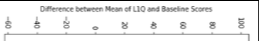
\includegraphics[width=4.5cm]{images/top.png}\\ 
			\vspace*{-1.35cm}\hspace{10em}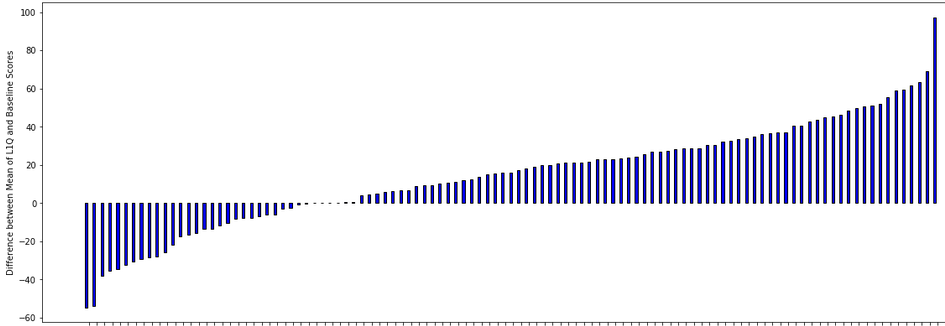
\includegraphics[width=21.3cm,height=4.5cm,angle=270]{images/resultsbarplot.png}
		\end{subfigure}
			\caption{The 109 metaphors used in the experiment, and baseline and $\protect\QLONE$ interpretations. Bar positions right of center indicate a preference for the pragmatic model.
			% This shows that for roughly 75\% of the metaphors, the $\protect\QLONE$ interpretation is preferred.
			}
			\label{fig:barplot}
		\end{figure}
		% todo: fix alignment stuff

		\citet{tsvetkov2014metaphor} provides a corpus of $\sim$800 AN metaphors, gathered by human annotators, from which we select $\sim$100 of the least frequent by bigram count\footnote{N-gram data from the Corpus of Contemporary American English \citep{davies2011word}.} for our experiment, in order to filter out conventionalized metaphors. Our full set of 109 metaphors is shown in figure \ref{fig:barplot}.

		In our experiment, each participant is shown a series of 12 metaphors, selected randomly from the total 109. For each metaphor, they are asked to rate on a slider four adjectives representing interpretations of the metaphor, of which two are selected by $\QLONE$ and two from a baseline model (details below). An example is shown in figure \ref{fig:slide}.

		The experiment was run on Mechanical Turk, with 99 participants, all of whom are native English speakers. Participants who failed to follow instructions on a test item were excluded, leaving 60 participants (analyses remain significant if all participants are included).
	
	\subsubsection{Baseline model}




		The aim of our experiment is to determine whether pragmatic reasoning results in better interpretations of metaphors, according to human judgments. As such, a natural baseline model to compare against is a model with a distributional semantics that does not make use of the pragmatic reasoning process inherent in $\QLONE$.

		Our baseline model is defined as follows: for a given metaphor of the form $(a$ $n)$, we take the mean of the adjective \emph{a} and noun \emph{n}. The two nearest (measured by cosine distance) adjectives $q$ to this mean are our baseline interpretations for the metaphor. We use the mean (a weighted sum) in light of the effectiveness of vector addition in deriving representations of phrasal and sentence meanings from constituent words \citep{mitchell2010composition,grefenstette2013category,socher2013recursive}. Cosine distance is a standard metric of similarity used for word embeddings \citep{pennington2014glove}.



			% relevant literature on vector addition / cosine:
			% 1. https://nlp.stanford.edu/~socherr/EMNLP2013_RNTN.pdf
			% 2. https://arxiv.org/pdf/1311.1539.pdf (section 2.3.1 onward)
			% 3. http://aclweb.org/anthology/E17-1006 (relevant to us)
			% 4. Much cited: https://onlinelibrary.wiley.com/doi/pdf/10.1111/j.1551-6709.2010.01106.x
			% Cosine distance for nearest neighbour:
			% https://nlp.stanford.edu/pubs/glove.pdf
			


	% \begin{figure}
	% 	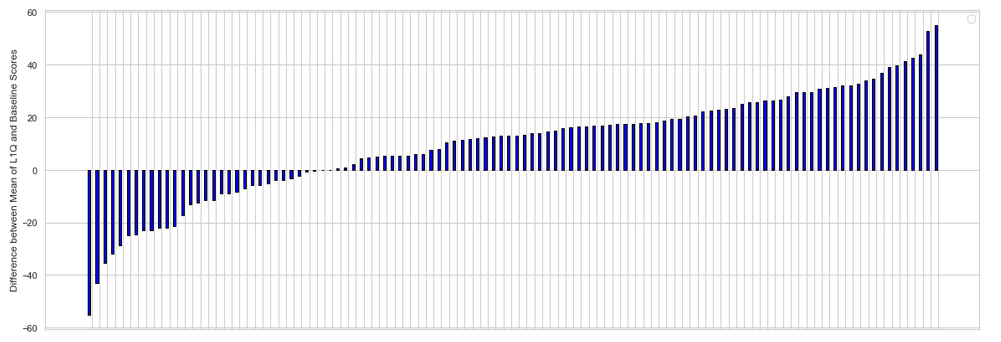
\includegraphics[height=5cm,angle=270,origin=c]{images/comparison1}


	% \end{figure}
	% \begin{figure}
	% 	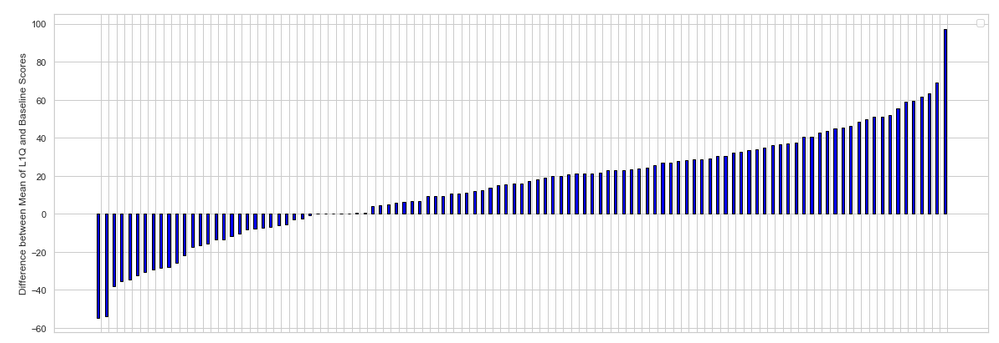
\includegraphics[height=5cm,angle=270,origin=c]{images/comparison2}	
	% \end{figure}



	\subsubsection{$\protect\QLONE$ hyperparameters}

		We use the largest available (300 dimensional) GloVe vectors, as our word embedding $E$. For each AN metaphor $(a$ $n)$, we specify $U$ as a set of 101 alternative utterances, consisting of $a$ and 100 of the nearest adjectives (by cosine distance) to $n$. These adjectives are chosen from the set of the 1425 adjectives with concreteness ranking $>3.0$ in the concreteness corpus of \citep{brysbaert2014concreteness}, to exclude abstract nouns.

		Similarly, we select a set $Q$ of projections corresponding to the hundred closest adjectives to the mean of the subject and predicate (the method of adjective choice in the baseline model), and take $P_{L_Q}$ to be a uniform distribution over $Q$. 

		By tuning on an independent validation set of hand-selected metaphors, we choose $\sigma_1=\sigma_2=0.1$. We select the adjectives corresponding to the two projections with highest marginal posterior mass under $\QLONE$ as the interpretations provided from our model in the experiment.
		% (the variances of the Gaussians used in the prior and semantics respectively). 

	\subsubsection{Analysis}

		The results, shown in figure \ref{fig:barplot}, were analyzed using a mixed-effects model with random slopes and intercepts for items and participants. The target interpretations were rated significantly higher than the baseline interpretations ($\beta$=13.8, $t$=5.3, p$<$0.001).


		
		% We ran a linear mixed effects model, predicting slider rating from baseline vs. $L_1$ metaphor, with by-metaphor and by-participant random intercepts. We find a significant correlation

			% As can be seen in Figure \ref{resultsbar}, there is a lot of variation in the average quality of proposed adjectives across both models, between metaphors. For the baseline model, we note that there is a subset of metaphors for which the baseline will perform well, as discussed in section (\ref{task1id}). These are metaphors where good projections $q$ are such that the subject and predicate are close when projected along $q$. In these cases, averaging the subject and predicate will generally give rise to a good interpretation. 
\section{Discussion} \label{conc} 

	We have shown that it is possible to scale Bayesian pragmatic reasoning to a distributional semantics and by so doing to obtain a model of metaphor interpretation. Our evaluation, the first such open domain test of an RSA model of interpretation, indicates that the principles of pragmatic reasoning continue to operate at this scale, and are key to obtaining human-like interpretations of metaphors. We see this as an important step towards a cognitively accurate and computationally tractable model of pragmatic language interpretation and production in general.

	%The significant improvement of $\QLONE$ over a model with the same semantics but no pragmatic reasoning provides evidence that this reasoning is key to obtaining human-like interpretations of metaphors.

	 

	% One direction of future work we consider to be especially promising is the extension of the system to multidimensional projections, since metaphors can plausibly convey multiple dimensions of meaning at once - in fact, we hypothesize that this is what motivates their use. We also aim to develop a pragmatic speaker $S_2$ as a model of metaphor production. More generally, optimization of our algorithm, in line with recent developments in word embeddings \citep{devlin2018bert,peters2018deep} should allow us to handle a broad range of metaphor in natural language. 
			% However, the model is extensible to the more general case, which we regard as an important direction for future work, since it allows us to capture the ability of metaphors to talk about many dimensions of meaning simultaneously.

	% valuable evidence that Gricean reasoning about informativity and relevance is key to the interpretation of metaphor, and language more generally.


		% DISCUSS UTTERANCES being finite set:
	% The prior for $S_1$, which is over possible utterances, is finite, and therefore straightforward to compute\footnote{As discussed in section \ref{rsa}, having a finite set of utterances is theoretically objectionable, but for the time being, a necessary modeling assumption.}. 
		% say that other RSA work attempts to relax this assumption, and that fusing the two is a direction for future work

	% optimization needed to make this nlp tool
	
	% On the one hand, we have developed a model of metaphor which performs well on a range of tasks. On the other, we have extended RSA to a distributional semantics, showing that the Bayesian approach to pragmatics can scale successfully to multidimensional continuous distributions. This scaling not only absolves the need for a hand-built semantics, but also for a hand-specified set of possible utterances and QUDs, since we can supply these both in a procedural way.

	% Of course, there are many ways in which the language which DistRSA models is not natural. For instance, we only treat very simple cases of metaphor, and model them in a way which ignores context, as well as the effect of words other than the subject and predicate. Furthermore, the speaker in our model has a finite set of possible utterances as a prior. This runs against basic theoretical insights regarding the productivity of language.

	% To address these shortcomings, a natural extension to our model would be the use of a neural speaker and listener (a direction pursued for simpler RSA models by \cite{andreas} and \cite{monroe2015learning}). Not only would this allow DistRSA to intake unprocessed language from an NL corpus, it would also result in a speaker who could produce potentially infinite utterances.
\bibliography{metaphor.bib}
\end{document}

